%% abtex2-modelo-trabalho-academico.tex, v-1.9.7 laurocesar
%% Copyright 2012-2018 by abnTeX2 group at http://www.abntex.net.br/
%%
%% This work may be distributed and/or modified under the
%% conditions of the LaTeX Project Public License, either version 1.3
%% of this license or (at your option) any later version.
%% The latest version of this license is in
%%   http://www.latex-project.org/lppl.txt
%% and version 1.3 or later is part of all distributions of LaTeX
%% version 2005/12/01 or later.
%%
%% This work has the LPPL maintenance status `maintained'.
%%
%% The Current Maintainer of this work is the abnTeX2 team, led
%% by Lauro César Araujo. Further information are available on
%% http://www.abntex.net.br/
%%
%% This work consists of the files abntex2-modelo-trabalho-academico.tex,
%% abntex2-modelo-include-comandos and abntex2-modelo-references.bib
%%

% ------------------------------------------------------------------------
% ------------------------------------------------------------------------
% abnTeX2: Modelo de Trabalho Academico (tese de doutorado, dissertacao de
% mestrado e trabalhos monograficos em geral) em conformidade com
% ABNT NBR 14724:2011: Informacao e documentacao - Trabalhos academicos -
% Apresentacao
% ------------------------------------------------------------------------
% ------------------------------------------------------------------------

\documentclass[
	% -- opções da classe memoir --
	12pt,				% tamanho da fonte
	openright,
	twoside,
	a4paper,			% tamanho do papel.
	% -- opções da classe abntex2 --
	% -- opções do pacote babel --
	english,			% idioma adicional para hifenização
	french,				% idioma adicional para hifenização
	spanish,			% idioma adicional para hifenização
	brazil				% o último idioma é o principal do documento
	]{abntex2}

\usepackage[T1]{fontenc}
\usepackage[utf8]{inputenc}
\usepackage{indentfirst}
\usepackage{color}
\usepackage{graphicx}
\usepackage{microtype}
\usepackage{amsmath}
\usepackage{amssymb}
\usepackage{ltablex}
\usepackage{subcaption}
\usepackage{pgfplots}
\pgfplotsset{width=10cm,compat=1.9}
\usepgfplotslibrary{external}
\usepgfplotslibrary{statistics}
\tikzexternalize
\usetikzlibrary{arrows.meta}
\usepackage{hhline}
\usepackage{array}
\usepackage{colortbl}
\usepackage{multirow}
\usepackage{placeins}
\usepackage{makecell}
\usepackage[brazilian,hyperpageref]{backref}
\usepackage[alf]{abntex2cite}

\makeatletter
\@addtoreset{chapter}{part}
\makeatother

\renewcommand{\backrefpagesname}{Citado na(s) página(s):~}
\renewcommand{\backref}{}
\renewcommand*{\backrefalt}[4]{
	\ifcase #1 %
		Nenhuma citação no texto.%
	\or
		Citado na página #2.%
	\else
		Citado #1 vezes nas páginas #2.%
	\fi}%

\newcommand{\oo}{\textordmasculine\ }

\newcommand{\tablemonofirst}[5]{%
	\renewcommand{\ArgX}{#1}
	\renewcommand{\ArgXI}{#2}
	\renewcommand{\ArgXII}{#3}
	\renewcommand{\ArgXIII}{#4}
	\renewcommand{\ArgXIV}{#5}
}

\newcommand{\tablemonosecond}[9]{%
	\begin{table}[h]
		\centering
		\caption{Análise dos dados para soluções de #1 e água}
		\label{#2}
		\bgroup
		\def\arraystretch{1.5}
		\scalebox{0.9}{%
		\begin{tabular}{| p{0.2\textwidth} | p{0.4\textwidth} | %
				p{0.4\textwidth} |}\hline
			\multirow{2}*{Composição} &
				\multicolumn{2}{c|}{Modelos}\\\hhline{~--}
			& Raoult & Virial\\\hhline{-~~}
			\multirow{5}*{\makecell[l]{Água,\\#1}} &
				$\frac{\sqrt{\sum\text{desvios}^2}}{n}=#3$ &
				$\frac{\sqrt{\sum\text{desvios}^2}}{n}=#4$%
					\\\hhline{~-~}
			& UNIQUAC & $b_\text{#1}=#9$\\\hhline{~~-}
			& $\frac{\sqrt{\sum\text{desvios}^2}}{n}=#5$ & Norrish\\
			& $q_\text{água}=\ArgXI$ &
				$\frac{\sqrt{\sum\text{desvios}^2}}{n}=#6$\\
			& $q_\text{#1}=\ArgXIII$ & $K_\text{#1}=\ArgX$%
				\\\hhline{-~~}
			$\bar{a_w}=#7$ & $u_\text{água}=\ArgXII$ & \\
			$\bar{x_w}=#8$ & $u_\text{#1}=\ArgXIV$ & \\\hline
		\end{tabular}}
		\egroup
	\end{table}
}

\newcommand{\tablebifirstzero}[9]{%
	\newcommand{\ArgX}{#1}
	\newcommand{\ArgXI}{#2}
	\newcommand{\ArgXII}{#3}
	\newcommand{\ArgXIII}{#4}
	\newcommand{\ArgXIV}{#5}
	\newcommand{\ArgXV}{#6}
	\newcommand{\ArgXVI}{#7}
	\newcommand{\ArgXVII}{#8}
	\newcommand{\ArgXVIII}{#9}
}
\newcommand{\tablebifirst}[9]{%
	\renewcommand{\ArgX}{#1}
	\renewcommand{\ArgXI}{#2}
	\renewcommand{\ArgXII}{#3}
	\renewcommand{\ArgXIII}{#4}
	\renewcommand{\ArgXIV}{#5}
	\renewcommand{\ArgXV}{#6}
	\renewcommand{\ArgXVI}{#7}
	\renewcommand{\ArgXVII}{#8}
	\renewcommand{\ArgXVIII}{#9}
}
\newcommand{\tabletrisecondzero}[9]{%
	\newcommand{\ArgXIX}{#1}
	\newcommand{\ArgXX}{#2}
	\newcommand{\ArgXXI}{#3}
	\newcommand{\ArgXXII}{#4}
	\newcommand{\ArgXXIII}{#5}
	\newcommand{\ArgXXIV}{#6}
	\newcommand{\ArgXXV}{#7}
	\newcommand{\ArgXXVI}{#8}
	\newcommand{\ArgXXVII}{#9}
}
\newcommand{\tablebisecond}[2]{%
	\renewcommand{\ArgXIX}{#1}
	\renewcommand{\ArgXX}{#2}
}

\newcommand{\tablebithird}[9]{%
	\begin{table}[h]
		\centering
		\caption{Análise dos dados para soluções de #1, #2 e água}
		\label{#3}
		\bgroup
		\def\arraystretch{1.5}
		\scalebox{0.9}{%
		\begin{tabular}{| p{0.2\textwidth} | p{0.4\textwidth} | %
				p{0.4\textwidth} |}\hline
			\multirow{2}*{Composição} &
				\multicolumn{2}{c|}{Modelos}\\\hhline{~--}
			& Raoult & Virial\\\hhline{-~~}
			\multirow{7}*{\makecell[l]{Água,\\#1 e\\#2}} &
				$\frac{\sqrt{\sum\text{desvios}^2}}{n}=#9$ &
				$\frac{\sqrt{\sum\text{desvios}^2}}{n}=#7$%
					\\\hhline{~-~}
			& UNIQUAC & $b_\text{#1}=\ArgX$\\
			& $\frac{\sqrt{\sum\text{desvios}^2}}{n}=#8$ &
				$b_\text{#2}=\ArgXI$\\
			& $q_\text{água}=\ArgXV$ &
				$c_\text{#1/#2}=\ArgXII$\\\hhline{~~-}
			& $q_\text{#1}=\ArgXVII$ & Norrish \\
			& $q_\text{#2}=\ArgXIX$ &
				$\frac{\sqrt{\sum\text{desvios}^2}}{n}=#6$ \\
			& $u_\text{água}=\ArgXVI$ & $K_\text{#1}=\ArgXIII$%
				\\\hhline{-~~}
			$\bar{a_w}=#4$ & $u_\text{#1}=\ArgXVIII$ &
				$K_\text{#2} = \ArgXIV$ \\
			$\bar{x_w}=#5$ & $u_\text{#2}=\ArgXX$ & \\\hline
		\end{tabular}}
		\egroup
	\end{table}
}

\newcommand{\tabletrifirst}[9]{%
	\renewcommand{\ArgX}{#1}
	\renewcommand{\ArgXI}{#2}
	\renewcommand{\ArgXII}{#3}
	\renewcommand{\ArgXIII}{#4}
	\renewcommand{\ArgXIV}{#5}
	\renewcommand{\ArgXV}{#6}
	\renewcommand{\ArgXVI}{#7}
	\renewcommand{\ArgXVII}{#8}
	\renewcommand{\ArgXVIII}{#9}
}

\newcommand{\tabletrisecond}[9]{%
	\renewcommand{\ArgXIX}{#1}
	\renewcommand{\ArgXX}{#2}
	\renewcommand{\ArgXXI}{#3}
	\renewcommand{\ArgXXII}{#4}
	\renewcommand{\ArgXXIII}{#5}
	\renewcommand{\ArgXXIV}{#6}
	\renewcommand{\ArgXXV}{#7}
	\renewcommand{\ArgXXVI}{#8}
	\renewcommand{\ArgXXVII}{#9}
}

\newcommand{\tabletrithird}[9]{%
	\begin{table}[h]
		\centering
		\caption{Análise dos dados para soluções de #1, #2, \ArgXXVII\ e água}
		\label{#3}
		\bgroup
		\def\arraystretch{1.5}
		\scalebox{0.9}{%
		\begin{tabular}{| p{0.2\textwidth} | p{0.4\textwidth} | %
				p{0.4\textwidth} |}\hline
			\multirow{2}*{Composição} &
				\multicolumn{2}{c|}{Modelos}\\\hhline{~--}
			& Raoult & Virial\\\hhline{-~~}
			\multirow{10}*{\makecell[l]{Água,\\#1,\\#2 e\\\ArgXXVII}} &
				$\frac{\sqrt{\sum\text{desvios}^2}}{n}=#9$ &
				$\frac{\sqrt{\sum\text{desvios}^2}}{n}=#7$%
					\\\hhline{~-~}
			& UNIQUAC & $b_\text{#1}=\ArgX$\\
			& $\frac{\sqrt{\sum\text{desvios}^2}}{n}=#8$ &
				$b_\text{#2}=\ArgXI$\\
			& $q_\text{água}=\ArgXIX$ & $b_\text{\ArgXXVII} = \ArgXIII$ \\
			& $q_\text{#1}=\ArgXXI$ &
				$c_\text{#2/#1}=\ArgXII$\\
			& $q_\text{#2}=\ArgXXIII$
				& $c_\text{\ArgXXVII/#1}=\ArgXIV$\\
			& $q_\text{\ArgXXVII}=\ArgXXV$
				& $c_\text{\ArgXXVII/#2}=\ArgXV$\\\hhline{~~-}
			& $u_\text{água}=\ArgXX$ & Norrish \\
			& $u_\text{#1}=\ArgXXII$ &
				$\frac{\sqrt{\sum\text{desvios}^2}}{n}=#6$ \\
			& $u_\text{#2}=\ArgXXIV$ & $K_\text{#1}=\ArgXVI$%
				\\\hhline{-~~}
			$\bar{a_w}=#4$ & $u_\text{\ArgXXVII}=\ArgXXVI$ &
				$K_\text{#2} = \ArgXVII$ \\
			$\bar{x_w}=#5$ & & $K_\text{\ArgXXVII}=\ArgXVIII$ \\\hline
		\end{tabular}}
		\egroup
	\end{table}
}

\tablebifirstzero{1}{1}{1}{1}{1}{1}{1}{1}{1}
\tabletrisecondzero{1}{1}{1}{1}{1}{1}{1}{1}{1}

\newcolumntype{C}{>{\centering\arraybackslash}p{3em}}
\newcolumntype{R}{>{\raggedleft\arraybackslash}X}
\newcolumntype{G}{>{\columncolor{lightgray}\centering\arraybackslash}p{3em}}

\DeclareMathOperator*{\minimize}{minimize}

\titulo{Relatório Final de Iniciação Científica/Tecnológica\\
	Modelagem Termodinâmica de Soluções de Interesse para a %
	Indústria de Alimentos}
\autor{Pedro Henrique Callil Soares}
\local{São Paulo}
\data{2021}
\orientador{Pedro de Alcântara Pessoa Filho}
\instituicao{%
	Universidade de São Paulo -- USP
	\par
	Escola Politécnica
	\par
	Departamento de Engenharia Química}
\tipotrabalho{Relatório de Iniciação Científica}
\preambulo{Relatório de projeto de iniciação científica/tecnológica
	- análise e modelagem da atividade da água em soluções de carboidratos
	e aminoácidos.}



\definecolor{blue}{RGB}{41,5,195}
\definecolor{pverydarkblue}{rgb}{0,0,0.2}
\definecolor{pdarkblue}{rgb}{0,0,0.4}
\definecolor{pblue}{rgb}{0,0,0.6}
\definecolor{pbrightblue}{rgb}{0,0,0.8}
\definecolor{pverybrightblue}{rgb}{0,0,1.0}
\definecolor{pverydarkred}{rgb}{0.15,0,0}
\definecolor{pdarkred}{rgb}{0.3,0,0}
\definecolor{pred}{rgb}{0.45,0,0}
\definecolor{pbrightred}{rgb}{0.6,0,0}
\definecolor{pverybrightred}{rgb}{0.75,0,0}
\definecolor{pviolindarkred}{rgb}{0.7,0.5,0.5}
\definecolor{pviolinred}{rgb}{0.8,0.5,0.5}
\definecolor{pviolinbrightred}{rgb}{0.9,0.5,0.5}
\definecolor{pviolindarkblue}{rgb}{0.5,0.5,0.7}
\definecolor{pviolinblue}{rgb}{0.5,0.5,0.8}
\definecolor{pviolinbrightblue}{rgb}{0.5,0.5,0.9}
\definecolor{pbackground}{rgb}{0.9,0.9,0.87}
\definecolor{pplanned}{rgb}{0.8,0.8,0.8}
\definecolor{pdoing}{rgb}{0.65,0.65,0.8}
\definecolor{pdone}{rgb}{0.5,0.5,0.8}


\makeatletter
\hypersetup{
		pdftitle={\@title},
		pdfauthor={\@author},
		pdfsubject={\imprimirpreambulo},
		pdfcreator={LuaLaTeX},
		pdfkeywords={atividade da água} {carboidratos} {aminoácidos},
		colorlinks=true,
		linkcolor=blue,
		citecolor=blue,
		filecolor=magenta,
		urlcolor=blue,
		bookmarksdepth=4
}
\makeatother

\makeatletter
\setlength{\@fptop}{5pt}
\makeatother

\newcommand{\quadroname}{Quadro}
\newcommand{\listofquadrosname}{Lista de quadros}

\newfloat[chapter]{quadro}{loq}{\quadroname}
\newlistof{listofquadros}{loq}{\listofquadrosname}
\newlistentry{quadro}{loq}{0}

\setfloatadjustment{quadro}{\centering}
\counterwithout{quadro}{chapter}
\renewcommand{\cftquadroname}{\quadroname\space}
\renewcommand*{\cftquadroaftersnum}{\hfill--\hfill}

\setfloatlocations{quadro}{hbtp}


\setlength{\parindent}{1.3cm}

\setlength{\parskip}{0.2cm}

\makeindex

\begin{document}

\selectlanguage{brazil}

\frenchspacing

\imprimircapa

\imprimirfolhaderosto


\setlength{\absparsep}{18pt}
\begin{resumo}
	Esse projeto tem o intuito de levantar uma base de dados sobre a
	atividade da água em soluções de carboidratos e aminoácidos,
	avaliando alguns modelos propostos com relação à sua capacidade
	correlativa com os dados experimentais. Foi feita uma revisão
	bibliográfica, levantando dados de atividade da água em função da
	composição para algumas soluções de interesse, e foram programadas
	rotinas computacionais visando avaliar os desvios entre os modelos,
	ajustados através de regressões não-lineares, e os dados. Por fim,
	foi feita uma análise da influência de diversos fatores na capacidade
	correlativa dos modelos examinados.\\
	\textbf{Palavras-chave}: soluções de carboidratos.
			soluções de aminoácidos.
			propriedades termodinâmicas de soluções.
			atividade da água.
			modelagem termodinâmica.
\end{resumo}

\pdfbookmark[0]{\listfigurename}{lof}
\listoffigures*
\cleardoublepage


\pdfbookmark[0]{\listtablename}{lot}
\listoftables*
\cleardoublepage

\begin{simbolos}
	\item[$ \gamma $] coeficiente de atividade
	\item[$ \phi $] coeficiente osmótico
	\item[$ \Pi $] pressão osmótica
	\item[$ a $] atividade
	\item[$ C_p $] calor específico
	\item[$ f $] fugacidade
	\item[$ \Delta H^\text{fus} $] Entalpia de vaporização
	\item[$ \Delta H^\text{vap} $] Entalpia de fusão
	\item[$ m $] molalidade
	\item[$ p^\text{vap} $] pressão de vapor
	\item[$ X_i $] fração mássica da substância $i$
	\item[$ x_i $] fração molar da substância $i$
	\item[$ \Xi_B, \Xi_F $] propriedade $\Xi$ no ponto de ebulição/congelamento
	\item[$ \Xi^\text{ID} $] propriedade $\Xi$ em um sistema ideal
	\item[$ \Xi^\text{ref} $] propriedade $\Xi$ no sistema de referência
	\item[$ \Xi_w $] propriedade $\Xi$ da água ($a_w, \gamma_w$, \textit{etc.} %
		para $\Xi = \alpha, \gamma$, \textit{etc.})
	\item[$K_i$] parâmetros do modelo de Norrish
	\item[$b_i$, $c_{ij}$] parâmetros do modelo virial
	\item[$q_i$, $u_{ii}$] parâmetros do modelo UNIQUAC
	\item[$A_i$] parâmetro de um modelo genérico
	\item[$\Phi$] Estimativa de coeficiente osmótico obtido através de %
		modelo genérico
\end{simbolos}

\pdfbookmark[0]{\contentsname}{toc}
\tableofcontents*
\cleardoublepage

\textual

\part{Introdução}

A atividade $a$ de uma substância, definida \cite{sandler2017} como
a razão entre a fugacidade de uma substância nas condições de um sistema
e sua fugacidade em uma situação de referência (equação \ref{eq:def_atv}),
age como sua ``concentração efetiva'', do ponto de vista termodinâmico.
Portanto, a medição e análise da atividade da água em soluções nos permite
prever de forma mais exata os fenômenos que dependem do teor de água em
um sistema. No caso da indústria de alimentos, o principal desses fenômenos
é a degradação dos alimentos por ação microbiana.

De fato, a grandeza que controla o crescimento microbiano em um alimento é a
atividade da água. No gráfico da figura \ref{fig:germ}\footnote{\cite{canovas2007}}
temos os valores de atividade da água necessários para a proliferação microbiana
para alguns microorganismos.

\begin{figure}[h]
	\centering
	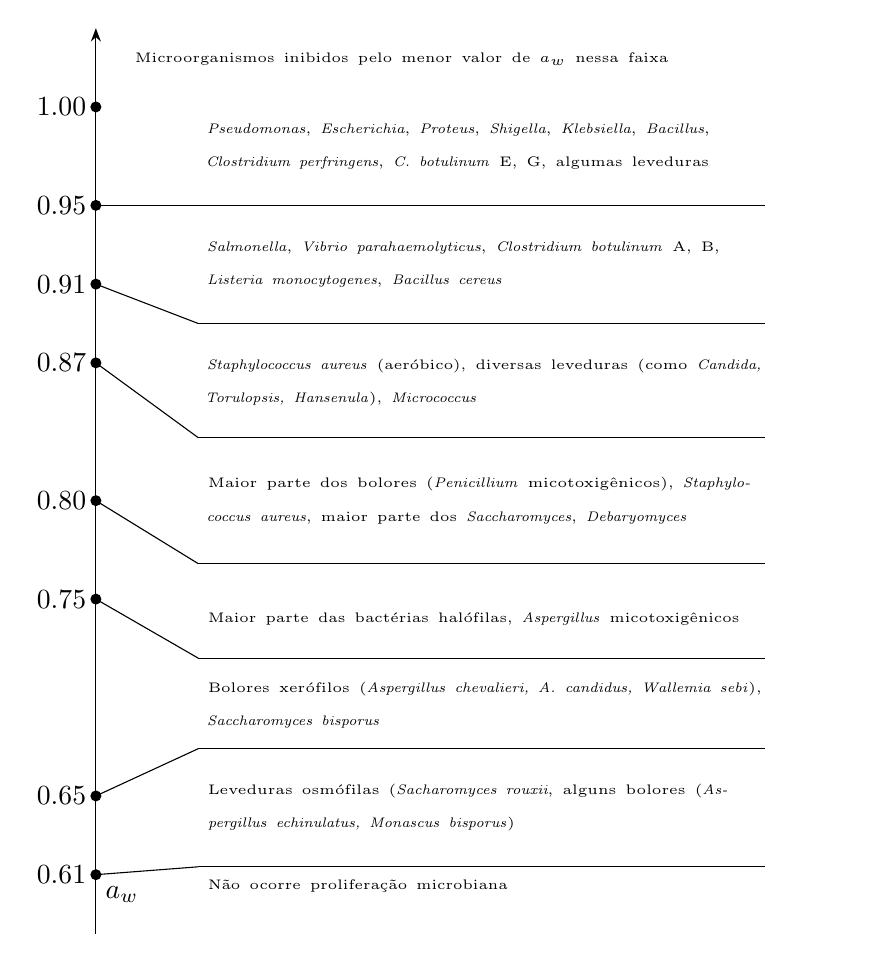
\begin{tikzpicture}[>=Stealth]
		\draw[->] (5,-0.5) -- (5,11);
		\draw (5,0.0) node[anchor=west] {$a_w$};
		\draw (5,8.75) -- (6.3,8.75);
		\draw (6.3,8.75) -- (13.5,8.75);
		\draw (5,7.75) -- (6.3,7.25);
		\draw (6.3,7.25) -- (13.5,7.25);
		\draw (5,6.75) -- (6.3,5.8);
		\draw (6.3,5.8) -- (13.5,5.8);
		\draw (5,5) -- (6.3,4.2);
		\draw (6.3,4.2) -- (13.5,4.2);
		\draw (5,3.75) -- (6.3,3);
		\draw (6.3,3) -- (13.5,3);
		\draw (5,1.25) -- (6.3,1.85);
		\draw (6.3,1.85) -- (13.5,1.85);
		\draw (5,0.25) -- (6.3,0.35);
		\draw (6.3,0.35) -- (13.5,0.35);
		\fill[black] (5,0.25) circle (0.07);
		\fill[black] (5,1.25) circle (0.07);
		\fill[black] (5,3.75) circle (0.07);
		\fill[black] (5,5) circle (0.07);
		\fill[black] (5,6.75) circle (0.07);
		\fill[black] (5,7.75) circle (0.07);
		\fill[black] (5,8.75) circle (0.07);
		\fill[black] (5,10) circle (0.07);
		\draw (10,10.4) node[anchor=south, text width=9cm]
		{\tiny{Microorganismos inibidos pelo menor valor de
		$a_w$ nessa faixa}};
		\draw (6.3,9.5) node[anchor=west, text width=7cm]
		{\tiny{\textit{Pseudomonas}, \textit{Escherichia},
		\textit{Proteus}, \textit{Shigella}, \textit{Klebsiella},
		\textit{Bacillus}, \textit{Clostridium perfringens},
		\textit{C. botulinum} E, G, algumas leveduras}};
		\draw (6.3,8) node[anchor=west, text width=7cm]
		{\tiny{\textit{Salmonella}, \textit{Vibrio parahaemolyticus},
		\textit{Clostridium botulinum} A, B, \textit{Listeria
		monocytogenes}, \textit{Bacillus cereus}}};
		\draw (6.3,6.5) node[anchor=west, text width=7cm]
		{\tiny{\textit{Staphylococcus aureus} (aeróbico), diversas
		leveduras (como \textit{Candida, Torulopsis, Hansenula}),
		\textit{Micrococcus}}};
		\draw (6.3,5) node[anchor=west, text width=7cm]
		{\tiny{Maior parte dos bolores (\textit{Penicillium}
		micotoxigênicos), \textit{Staphylococcus aureus},
		maior parte dos \textit{Saccharomyces}, \textit{Debaryomyces}}};
		\draw (6.3,3.5) node[anchor=west, text width=7cm]
		{\tiny{Maior parte das bactérias halófilas, \textit{Aspergillus}
		micotoxigênicos}};
		\draw (6.3,2.4) node[anchor=west, text width=7cm]
		{\tiny{Bolores xerófilos (\textit{Aspergillus chevalieri, A.
		candidus, Wallemia sebi}), \textit{Saccharomyces bisporus}}};
		\draw (6.3,1.1) node[anchor=west, text width=7cm]
		{\tiny{Leveduras osmófilas (\textit{Sacharomyces rouxii},
		alguns bolores (\textit{Aspergillus echinulatus, Monascus
		bisporus})}};
		\draw (6.3,0.1) node[anchor=west, text width=7cm]
		{\tiny{Não ocorre proliferação microbiana}};
		\draw (5,0.25) node[anchor=east] {0.61};
		\draw (5,1.25) node[anchor=east] {0.65};
		\draw (5,3.75) node[anchor=east] {0.75};
		\draw (5,5) node[anchor=east] {0.80};
		\draw (5,6.75) node[anchor=east] {0.87};
		\draw (5,7.75) node[anchor=east] {0.91};
		\draw (5,8.75) node[anchor=east] {0.95};
		\draw (5,10) node[anchor=east] {1.00};
	\end{tikzpicture}
	\caption{Valores de $a_w$ para o crescimento microbiano}
	\label{fig:germ}
\end{figure}

Nas condições encontradas na indústria de alimentos, não é absurdo assumir a
hipótese de gás ideal para a fase gás dos sistemas
considerados \cite{canovas2007}, em muitas situações. Além disso, a condição de
referência é tomada como água pura, líquida, à mesma temperatura $T$. Assim
obtemos:

\begin{equation}
	\label{eq:def_atv}
	a_w \equiv \left(\cfrac{f_w}{f^\text{ref}_w}\right)_T%
		\approx \left(\cfrac{p^\text{vap}_w}{p^\text{vap,ref}_w}\right)_T
\end{equation}

Para soluções ideais, obter $a_w$ é simples: para todo componente $i$ da
mistura, a sua atividade é dada, simplesmente por sua fração molar, e portanto
$a_w = x_w$. Entretanto, essa hipótese nem sempre se verifica; assim sendo,
para soluções ideais adotamos o coeficiente de atividade $\gamma_w$:

\begin{equation}
	a_w = \gamma_wx_w \implies \gamma_w = \cfrac{a_w}{x_w}
\end{equation}

Entretanto, ainda que o coeficiente de atividade seja um indicador para o
desvio da idealidade em uma solução, apresenta um problema: é uma grandeza ruim
para avaliarmos os desvios da idealidade em soluções diluídas, já que, sendo
$a_w$ função contínua da fração molar de água, e dado que a atividade da água
pura é de 1 (é, afinal, a solução de referência), temos que:

\begin{equation}
	\lim_{x_w \to 1}\gamma_w = 1
\end{equation}

E, para muitas soluções de interesse, não somente temos altos desvios da
idealidade, como também temos soluções extremamente diluídas. Então adotamos
uma nova grandeza, o coeficiente osmótico $\phi$, dado por:

\begin{equation}
	\phi = \cfrac{\ln(a_w)}{\ln(x_w)}
\end{equation}

Para comparar essas grandezas e visualizar um possível comportamento da
atividade da água com a mudança na composição de uma substância, podemos
observar o gráfico na figura \ref{fig_atv_gamma_gluc} \cite{ebrahimi2016}.

\begin{figure}[h]
	\centering
	\begin{tikzpicture}
		\newsavebox{\minigrafglic}
		\savebox{\minigrafglic}{%
		\scalebox{0.5}{%
		\begin{tikzpicture}
			\begin{axis}[
			xmin=0.97,xmax=1.0,
			ymin=0.97,ymax=1.0,
			x dir=reverse,
			width=7cm,
			height=7cm,
			xlabel = {$x_w$},
			ylabel = {$a_w$},
			]
			\addplot+[
				color=pverydarkred,
				mark=o,
				only marks,
			]
			table[x={xw},y={aw}]{glucose_a_w_and_phi.dat};
			\addlegendentry{$a_w$ experimental};
			\addplot+[
				color=black,
				no marks,
				domain=0.96:1.0,
				samples=5,
			]{x};
			\addlegendentry{$a_w=x_w$};
		\end{axis}
	\end{tikzpicture}
	}}
	\begin{axis}[
			xmin = 0.97, xmax = 1.0, xlabel = {$x_w$},
			ymin = 0.96, ymax = 1.05, ylabel = {$\phi$},
			x tick label style={
				/pgf/number format/.cd,
				fixed,
				fixed zerofill,
				precision=3,
				/tikz/.cd
			},
			y tick label style={
				/pgf/number format/.cd,
				fixed,
				fixed zerofill,
				precision=3,
				/tikz/.cd
			},
			legend pos = south west,
			axis y line=left,
			x axis line style={-},
			xlabel near ticks,
			ylabel near ticks,
			x dir=reverse,
			ytick={0.97,0.985,1.00,1.015,1.03,1.045},
		]
		\addplot+[
			color=pdarkblue,
			mark=square,
			very thick,
			only marks,
		]
		table[x={xw},y={phi}]{glucose_a_w_and_phi.dat};
		\addlegendentry{$\phi$};
		\draw (axis cs: 0.981,0.99)node{\usebox{\minigrafglic}};
		\end{axis}
		\begin{axis}[
			xmin = 0.97, xmax = 1.0, xlabel = {$x_w$},
			ymin = 0.9977, ymax = 1.0001, ylabel = {$\gamma_w$},
			y tick label style={
				/pgf/number format/.cd,
				fixed,
				fixed zerofill,
				precision=4,
				/tikz/.cd
			},
			axis y line=right,
			axis x line=none,
			legend pos = south east,
			x dir=reverse,
		]
		\addplot+[
			color=pverybrightred,
			mark=o,
			very thick,
			only marks,
		]
		table[x={xw},y={gammaw}]{glucose_a_w_and_phi.dat};
		\addlegendentry{$\gamma_w$};
		\end{axis}
	\end{tikzpicture}
	\caption{Atividade ($a_w$), coeficiente de atividade ($\gamma_w$) e%
	coeficiente osmótico ($\phi$) da água em soluções de D-glicose. %
	Perceba a diferença entre as escalas utilizadas para $\gamma_w$ e $\phi$.}
	\label{fig_atv_gamma_gluc}
\end{figure}

Devemos, além disso, lembrar que a medida de atividade da água é, por vezes,
realizada de modo mais indireto; podemos medir para uma determinada solução ao
invés de seu valor de atividade da água (através da medição de sua pressão de
vapor e comparação com a pressão de vapor de água pura nas mesmas condições), o
seu valor de elevação do ponto de ebulição, de depressão de ponto de início de
congelamento, ou a composição de uma outra solução em equilíbrio osmótico.

Por exemplo, alguns conjuntos de dados obtidos para soluções $n$-árias de
carboidratos \cite{abderafi1994} apresentam dados de elevação do ponto de
ebulição. Essas medidas devem ser convertidas em dados de coeficiente osmótico,
através das equações \ref{eq:eleb_to_osco} \cite{ge2009,ge2009err}, por
exemplo, que estão exibidas na figura \ref{fig_ge_and_wang}.

\begin{equation}
	\label{eq:eleb_to_osco}
	\begin{cases}
		\ln(a_w) = -\cfrac{\Delta H^\text{vap}_{0,T_B}\left(\cfrac{1}{T_B}%
			-\cfrac{1}{T_B+\Delta T_B}\right)-%
			\Delta C_p^\text{vap}\Bigg[\ln\left(\cfrac{T_B+%
			\Delta T_B}{T_B}\right) - \cfrac{\Delta T_B}{T_B+%
			\Delta T_B}\Bigg]}{R}\\
		\ln(a_w) = \cfrac{\Delta H^\text{fus}_{0,T_F}\left(\cfrac{1}{T_F}-%
		\cfrac{1}{T_F-\Delta T_F}\right)+\Delta C_p^\text{fus}%
		\Bigg[\ln\left(\cfrac{T_F-\Delta T_F}{T_F}\right) -%
		\cfrac{\Delta T_F}{T_F-\Delta T_F}\Bigg]}{R}
	\end{cases}
\end{equation}

\begin{figure}[h]
	\centering
	\begin{subfigure}{0.5\textwidth}
		\begin{tikzpicture}[scale=0.75]
			\begin{axis}[
				ylabel={$a_w$},
				xlabel={$T_B$[\textcelsius]},
				ymax=1, xmax=115, xmin=100,
			]
				\addplot [
					color=pred,
					no marks,
					very thick,
				]
					table [x={BPE},y={aw},col sep=comma]
						{ge_and_wang_bpe.csv};
			\end{axis}
		\end{tikzpicture}
		\caption{Ponto de Ebulição}
	\end{subfigure}%
	\hfill%
	\begin{subfigure}{0.5\textwidth}
		\begin{tikzpicture}[scale=0.75]
			\begin{axis}[
				ylabel={$a_w$},
				xlabel={$T_F$[\textcelsius]},
				ymax=1, xmin=-15, xmax=0,
			]
				\addplot [
					color=pblue,
					no marks,
					very thick,
				]
					table [x={FPD},y={aw},col sep=comma]
						{ge_and_wang_fpd.csv};
			\end{axis}
		\end{tikzpicture}
		\caption{Ponto de Fusão}
	\end{subfigure}
	\caption{Relações entre $T_B$/$T_F$ (em \textcelsius) e $a_w$, %
		$P=P_\text{atm}$}
	\label{fig_ge_and_wang}
\end{figure}

Com $\Delta C_p$ sendo definido como a diferença entre os calores
específicos, entre as fases: $\Delta C_p^\text{vap} = C_p^\text{vapor} -%
C_p^\text{líquido}$ e $\Delta C_p^\text{fus} = C_p^\text{líquido} -%
C_p^\text{sólido}$, $\Delta T_F$ sendo a depressão do ponto de congelamento,
$\Delta T_B$ a elevação do ponto de ebulição e $\Delta H_{0,T_F}^\text{vap}$ e
$\Delta H_{0,T_F}^\text{fus}$ sendo as entalpias de vaporização e ebulição do
solvente puro a $T_F$.

\part{Revisão Bibliográfica}

\chapter{Modelagem da atividade da água}

\section{Modelos avaliados}

Foram analisados diversos modelos, desde mais simples como a Lei de Raoult ou
equação de Caurie a mais complexos como o método iterativo originário da equação
de Zdanovskii, para posterior comparação com uma equação do tipo virial (equação
como \ref{eq:ad_pessoa}, a adaptada de \cite{pessoa2008}, na qual $b_i$ e
$c_{ij}$ são parâmetros ajustáveis e $\theta_i$ é uma medida de concentração,
com $i,j$ componentes da mistura).

\begin{equation}
	\label{eq:ad_pessoa}
	\ln(a_w) = \sum_{i \neq w}\theta_i\Bigg(1 +%
	2b_i+3\sum_{j \neq w}c_{ij}\theta_j\Bigg)
\end{equation}

Para obter os valores de $a_w$ para soluções com apenas um soluto, temos
diversos modelos que podem ser aplicados. Desses, serão analisados e comparados
os seguintes:

\begin{itemize}
	\item Lei de Raoult: Modelo mais simples, para soluções ideais. Assume
		atividade da água $a_w = x_w$, sua fração molar;
	\item Equação de Norrish \cite{norrish1966}: correção da lei de Raoult.
		Sendo $x_w$ a fração molar da água e $x_s$ a do soluto e
		tomando uma constante $K$, experimental, temos a equação
		\ref{eq_norrish}:
		\begin{equation}
			\label{eq_norrish}
			a_w = x_w\exp\Big[\Big(\sqrt{K}x_s\Big)^2\Big]
		\end{equation}
	\item Modelo UNIQUAC (\textit{universal quasi-chemical})
		\cite{abrams1975} Modelo mais refinado dentre os avaliados no
		projeto, demanda dois parâmetros para o ajuste para cada par de
		componentes da mistura (solvente e solutos), podendo ser tanto
		utilizado para sistemas binários quanto para sistemas $n$-ários.
		Embora claramente apresente custo computacional elevado para
		misturas com muitos componentes (já que o número de parâmetros
		é da ordem do número de componentes ao quadrado), os dados
		utilizados não são de misturas complexas o suficiente para que
		isso seja um problema.
\end{itemize}

Os modelos considerados para análise e comparação serão, para sistemas
multicomponente, os seguintes:

\begin{itemize}
	\item Lei de Raoult: atividade da água $a_w$ sendo igual a $x_w$,
		sua fração molar;
	\item Equação de Norrish: adotada pequena modificação para equação
		\ref{eq_norrish}, como visto na equação \ref{eq_norrish_multi};
		\begin{equation}
			\label{eq_norrish_multi}
			a_w = x_w\exp\Big[\Big(\sum_{i \neq w}%
			\sqrt{K_i}x_i\Big)^2\Big]
		\end{equation}
	\item Modelo de Caurie \cite{caurie1986}: atividade da água como uma
		correção do produto das atividades da água para uma solução
		com um único componente (equação \ref{eq_caurie}) com
		$m_i$ a molalidade do componente $i$ em solução, $a_{wi}$
		sendo a atividade da água em uma mistura com o componente
		$i$, apenas, tal que $m_i$ se mantenha e $n$ sendo o número de
		componentes em solução.
		\begin{equation}
			\label{eq_caurie}
			a_w = \prod_{i \neq w}a_{wi}-\left[\cfrac{n}%
			{55.5^2}\sum_{\substack{i \neq j \\ i,j \neq w}}%
			m_im_j + \cfrac{(n+1)}{55.5^3}\sum_{%
			\substack{i\neq j,k \\ j \neq k \\  i,j,k \neq w}}%
			m_im_jm_k\right]
		\end{equation}
		Para a obtenção das atividades da água de substâncias
		binárias, foi utilizada a Lei de Raoult.
	\item Relação de Zdanovskii \cite{chen1973,sangster1973}:
		para uma mistura ternária composta por água e mais dois
		componentes, digamos, 1 e 2, adotamos duas soluções binárias,
		cada uma com um componente, em equilíbrio osmótico com uma
		terceira, ternária. Sendo $m_{01}$ e $m_{02}$ as
		molalidades do componente 1 na solução na qual é o único
		soluto e do componente 2 na solução no qual é o único soluto, e
		sendo $m_1$ e $m_2$ as molalidades de 1 e 2 na solução ternária,
		temos que $m_1m_{01}^{-1} + m_2m_{0_2}^{-1} = 1$, sendo esta a
		relação de Zdanovskii. Disso se obtém um procedimento iterativo,
		que possibilita obter, tendo as isotermas de cada componente, a
		atividade da água de uma mistura ternária.
	\item Modelo UNIQUAC (\textit{universal quasi-chemical}), citado
		anteriormente.
\end{itemize}

\section{Aplicabilidade das amostras aos modelos}

Como não temos interesse apenas em ajustar curvas aos dados para sistemas
$n$-ários, mas também queremos avaliar a possibilidade de prever coeficientes
osmóticos para esses sistemas a partir de dados obtidos do ajuste de sistemas
binários, podemos dividir os modelos estudados em dois grandes grupos. Sendo um
modelo termodinâmico a $N$ parâmetros $(A_j)_{j \in \{1, 2, \ldots N\}}$ para o
coeficiente osmótico em um sistema de composição $(x_i)_\text{$i$ componente}$,
com temperatura $T$ e pressão $P$ dado pela equação \ref{eq:geral_bigphi},
podemos obter aproximações para os parâmetros $(A_j^*)_{j \in \{1, 2, \ldots, N\}}$
a partir do método dos mínimos quadrados, dado na expressão \ref{eq:min_quad},
para um conjunto de $K$ dados experimentais $\{(\phi^k, T^k, P^k,%
	(x_i)^k_\text{$i$ componente}), k \in \{1,2,\ldots,K\}\}$.

\begin{equation}
	\label{eq:geral_bigphi}
	\phi = \Phi((A_j)_{j \in \{1, 2, \ldots, N\}}, (x_i)_\text{$i$ %
		componente da mistura}, T, P)
\end{equation}

\begin{equation}
	\label{eq:min_quad}
	\minimize_{(A_j^*)_{j \in \{1,2,\ldots,N\}} \in \mathbb{R}^N}%
	\left(\sum_{k \in \{1,2,\ldots,K\}}\left[\phi^k - \Phi((A^*_j)_{j%
	\in \{1, 2, \ldots, N\}}, (x^k_i)_\text{$i$ componente},%
	T^k, P^k)\right]^2\right)
\end{equation}

Para dados obtidos exclusivamente de sistemas binários, temos que:

\begin{equation}
	\forall k \in \{1,2,\ldots,K\} \;\; \exists i \neq w%
	\text{ componente } : \forall \;\; i' \neq i, i' \neq w\;\; x^k_{i'} = 0
\end{equation}

Quando para todo conjunto de dados obtidos exclusivamente de sistemas binários
temos que é válida a expressão \ref{eq:no_bin_fit},
dizemos que o modelo apresenta parâmetro ajustável de interação entre os
solutos. Caso contrário, dizemos que o modelo não apresenta parâmetro
ajustável de interação entre os solutos.

\begin{equation}
	\label{eq:no_bin_fit}
	\exists j' \in \{1,2,\ldots,N\} : \forall \alpha \in \mathbb{R}\;\;%
	(A_j^*)_{j \in \{1,2,\ldots,N\}, A_{j'}^* = \alpha}%
	\text{ é solução de \ref{eq:min_quad}}
\end{equation}

Essa distinção se faz necessária a um dos objetivos do projeto, a saber, avaliar
a aplicabilidade de parâmetros obtidos a partir do ajuste de um modelo a dados
de sistemas binários à predição de dados de sistemas $n$-ários, aplicabilidade
essa que, caso verificada, traria grande vantagem ao modelo em questão, tendo em
vista a quantidade de dados disponível para um sistema binário qualquer
ser muito superior à quantidade de dados disponível para um sistema $n$-ário
qualquer. Além disso, também deve-se levar em conta que os experimentos de
laboratório necessários ao levantamento de dados representativos para sistemas
$n$-ários são muito mais custosos.

É exemplo de modelo da segunda categoria o proposto por Norrish; para a
primeira categoria, mais complexa, o modelo do tipo virial proposto na equação
\ref{eq:ad_pessoa} pode ser citado como exemplo. Além disso, claramente temos,
inclusos de forma trivial na segunda categoria, modelos sem parâmetro ajustável
algum, como a Lei de Raoult. Esses modelos mais simples devem, também, ser
separados para avaliação de seu poder preditivo.

\section{Limitações dos modelos e principais problemas encontrados}

Um dos principais problemas encontrados é a simples não aplicabilidade de
alguns modelos em determinadas situações: para exemplificar essa situação,
analisaremos o modelo de Norrish e suas limitações intrínsecas.

O modelo de Norrish, como visto em \ref{eq_norrish} e \ref{eq_norrish_multi},
apresenta a equação \ref{eq_phi_norrish} para o cálculo do coeficiente
osmótico $\phi$:

\begin{equation}
	\label{eq_phi_norrish}
	\phi = \cfrac{\ln(a_w)}{\ln(x_w)} = \cfrac{\ln(x_w) + \left(\sum_{ i\neq w}
	\sqrt{K_i}x_1\right)^2}{\ln(x_w)}
\end{equation}

Como $x_w \le 1 \implies \ln(x_w) \le 0$, temos que o modelo prevê apenas
valores do coeficiente osmótico menores que 1. Isso definitivamente não se
verifica nos dados reais: temos diversos comportamentos possíveis, desde
dados que se assemelham a funções monótonas decrescentes, como exigido pelo
modelo,\footnote{%
	Já que $\lim_{x_w \to 1}\phi_\text{Norrish} = 1$.
} até dados que se assemelham a funções monótonas crescentes, o oposto do
desejado. Isso pode ser visto na própria figura \ref{fig_atv_gamma_gluc}, e,
mais claramente, na figura \ref{fig_manose_phi}.

Outro exemplo é a equação de Caurie: como $\lim_{x_w \to 0}m_i = +\infty$,
temos que existem concentrações a partir das quais o modelo simplesmente não
retorna resultados físicos, já que $a_w \in [0,1]$ e, como exibido na equação
\ref{eq_caurie_fail}, existem certos valores para as frações molares de cada
componente na mistura que retornam valores negativos de $a_{w,\text{Caurie}}$.
Além disso, conforme a fração molar de água na mistura decresce, $\phi$ deve
se aproximar de 0, no limite.

\begin{equation}
	\label{eq_caurie_fail}
	\begin{split}
		a_{w,\text{Caurie}} = \prod_{i \neq w}a_{w,i} - \left[\cfrac{n}%
			{55.5^2}\sum_{\substack{i \neq j \\ i,j \neq w}}%
			m_im_j + \cfrac{(n+1)}{55.5^3}\sum_{%
			\substack{i\neq j,k \\ j \neq k \\  i,j,k \neq w}}
			m_im_jm_k\right] <\\
		1 - \cfrac{n}{55.5^3}\left[55.5 \times%
			\sum_{\substack{i \neq j \\ i,j \neq w}}%
			m_im_j + \cfrac{n+1}{n}\sum_{%
			\substack{i\neq j,k \\ j \neq k \\  i,j,k \neq w}}
			m_im_jm_k\right]\implies\\
		\lim_{\substack{m_k \to +\infty \\%
				\forall n \neq k, \text{ $m_n$ constante}}}%
			a_{w,\text{Caurie}} = -\infty \implies%
		\lim_{x_w \to 0} a_{w,\text{Caurie}} = -\infty
	\end{split}
\end{equation}

Essa diversidade de comportamentos pode vir a ser útil. Por exemplo, para o
modelo virial, a medida de concentração escolhida foi a concentração molar, já
que é possível demonstrar que os dados dificilmente seguem a forma à qual são
restritos ao utilizarmos a fração molar (mais intuitiva) como medida. Isso pode
ser visto na equação \ref{eq_phi_virial_mono_frac}
\footnote{%
	Podemos afirmar isso já que temos, $\forall w > 0$:
	\begin{equation*}
		\begin{split}
			e^w = 1 + w + \cfrac{w^2}{2!} + \ldots \ge w +1
			\stackrel{(z = w+1)}{\implies} e^z \ge ze \implies
				z \ge \ln(z) + 1
			\stackrel{\left(y=\cfrac{1}{z}\right)}{\implies}
				\cfrac{1}{y} \ge
				\ln\left(\cfrac{1}{y}\right) + 1 \implies\\
			1-y \ge y\ln\left(\cfrac{1}{y}\right)
			\stackrel{(x=1-y)}{\implies} x >
				(1-x)\ln\left(\cfrac{1}{1-x}\right)\implies
			\cfrac{x}{1-x} + \ln(1-x) > 0 \implies\\
				\cfrac{d}{dx}\left(\cfrac{x}{\ln(1-x)}\right) > 0
		\end{split}
	\end{equation*}
}
para sistemas binários, sendo $x$ a fração molar do soluto: o modelo (com
$\theta_i = x_i$) implica em uma função monótona.

\begin{equation}
	\label{eq_phi_virial_mono_frac}
	\begin{split}
		\ln(a_w) = -x + 2bx \implies \phi =
			\cfrac{-x + 2bx}{\ln(1-x)}\implies\\
		\phi = (2b-1)\cfrac{x}{\ln(1-x)} \implies
			\forall (x_1,x_2) \in (0,1)\times(0,1)\;\;
			\cfrac{d\phi}{dx}\Big|_{x_1} \times
			\cfrac{d\phi}{dx}\Big|_{x_2} \ge 0
	\end{split}
\end{equation}

Outro problema (não intrínseco aos modelos, mas específico aos dados) é a
existência de pequenos conjuntos de dados, comparados ao que seria
necessário para ajustar o modelo UNIQUAC completo, por exemplo. De fato,
para uma mistura que, seja composta por $n$ substâncias, o modelo exige
$2n+n^2 \in \mathcal{O}(n^2)$ parâmetros (para contabilizar as energias de
interação $U_{ij}$ e os parâmetros $r_i$ e $q_i$). Dessa forma, algumas
simplificações (equações exibidas em \ref{eq_uniquac_simpl}), presentes
na literatura, foram adotadas.

\begin{equation}
	\label{eq_uniquac_simpl}
	\begin{cases}
		u_{ij} = \sqrt{u_{ii}u_{jj}}\\
		r_i = q_i
	\end{cases}\forall\ i, j\text{ componente}
\end{equation}

Devemos lembrar, além disso, que boa parte dos comjuntos de dados para sistemas
multicomponente apresenta problemas com colinearidade; isso não prejudica a
predição de novos dados, mas torna pouco confiáveis os valores obtidos para os
parâmetros. Por fim, existem problemas quanto a precisão dos dados de coeficiente
osmótico, como já discutido.


\begin{figure}[h]
	\centering
	\begin{tikzpicture}
		\newsavebox{\minigrafmann}
		\savebox{\minigrafmann}{%
		\scalebox{0.5}{%
		\begin{tikzpicture}
			\begin{axis}[
			xmin=0.0,xmax=0.07,
			ymin=0.93,ymax=1.0,
			width=7cm,
			height=7cm,
			xlabel = {$x$},
			ylabel = {$a_w$},
			xlabel near ticks,
			ylabel near ticks,
			xticklabel style={
				/pgf/number format/fixed,
				/pgf/number format/precision=3,
				/pgf/number format/fixed zerofill
			},
			scaled x ticks=false,
			]
			\addplot+[
				color=pbrightred,
				mark=o,
				only marks,
				thick,
			]
			table[x={mannose},y={aw_exp},col sep=comma]
				{ebrahimi_mannose_norrish.csv};
			\addplot+[
				color=pverybrightblue,
				no marks,
				thick,
			]
			table[x={mannose},y={aw_calc},col sep=comma]
				{ebrahimi_mannose_norrish.csv};
			\addplot+[
				color=pblue,
				no marks,
				thick,
			]
			table[x={mannose},y={aw_calc},col sep=comma]
				{ebrahimi_mannose_virial.csv};
			\addplot+[
				color=pverydarkblue,
				no marks,
				thick,
			]
			table[x={mannose},y={aw_calc},col sep=comma]
				{ebrahimi_mannose_uniquac.csv};
		\end{axis}
	\end{tikzpicture}
	}}
	\begin{axis}[
			xmin = 0.0, xmax = 0.072, xlabel = {$x_\text{mannose}$},
			ymin = 0.975, ymax = 1.029, ylabel = {$\phi$},
			legend pos = south east,
			xlabel near ticks,
			ylabel near ticks,
			xticklabel style={
				/pgf/number format/fixed,
				/pgf/number format/precision=3,
				/pgf/number format/fixed zerofill
			},
			scaled x ticks=false,
			xtick = {0.015,0.030,0.045,0.060},
		]
		\addplot+[
			smooth,
			color=pverybrightblue,
			no marks,
			thick,
		]
		table[x={mannose},y={phi_calc},col sep=comma]
			{ebrahimi_mannose_norrish.csv};
		\addlegendentry{Norrish};
		\addplot+[
			smooth,
			color=pblue,
			no marks,
			thick,
		]
		table[x={mannose},y={phi_calc},col sep=comma]
			{ebrahimi_mannose_virial.csv};
		\addlegendentry{virial};
		\addplot+[
			smooth,
			color=pverydarkblue,
			no marks,
			thick,
		]
		table[x={mannose},y={phi_calc},col sep=comma]
			{ebrahimi_mannose_uniquac.csv};
		\addlegendentry{UNIQUAC};
		\addplot+[
			color=pbrightred,
			mark=o,
			very thick,
			only marks,
		]
		table[x={mannose},y={phi_exp},col sep=comma]
			{ebrahimi_mannose_uniquac.csv};
		\addlegendentry{experimental};
		\draw (axis cs:0.018,1.015) node{\usebox{\minigrafmann}};
		\end{axis}
	\end{tikzpicture}
	\caption{Coeficiente osmótico $\phi$ e ajuste de modelos
		para solução de manose}
	\label{fig_manose_phi}
\end{figure}


\chapter{Seleção de dados experimentais}

\label{sec_selec_data}

Devido às presentes circunstâncias, não é prático ou seguro fazer experimentos
laboratoriais para levantamento de dados. Felizmente, também não é necessário:
a literatura científica sobre o assunto é extensa o suficiente para possibilitar
a obtenção uma boa seleção de dados experimentais previamente publicados, para
sistemas multicomponente e binários, que se encontram resumidos nas listas e
tabelas que seguem.

\begin{itemize}
	\item Para sistemas binários:
		\begin{itemize}
			\item Abderafi \& Bounahmidi (1994) \cite{abderafi1994};
			\item Bhandari \& Bareyre (2003) \cite{bhandari2003},
				medidas diretas de $a_w$ para soluções de água
				e glicose a 25\textcelsius, com valores entre
				$x_w = 0.808$ e $x_w = 0.917$;
			\item Bonner (1982) \cite{bonner1982}, medidas de
				coeficiente osmótico e de atividade para lisina
				e arginina a temperatura de 298.15K.
			\item Chen (1987) \cite{chen1987}, medidas para atividade
				de água de algumas soluções de carboidratos obtidas
				a partir de dados de umidade relativa de equilíbrio,
				à temperatura de congelamento.
			\item Cooke, Jónsdóttir \& Westh (2002) \cite{cooke2002a},
				medidas de pressão de vapor em temperaturas de
				24.91\textcelsius, para a sacarose, e
				44.84\textcelsius, para frutose, e outros
				carboidratos, com frações molares entre 0 e 0.24 a
				depender da substância.
%			\item Dunning, Evans \& Taylor (1951) \cite{dunning1951},
%				medidas de pressão de vapor da água para soluções de
%				sacarose com temperaturas entre 60 e
%				95\textcelsius\ e frações molares $x_w$ entre 0.79
%				e 0.96.\footnote{%
%					Não puderam ser utilizados, tendo em vista
%					que foram, todos, obtidos a temperaturas
%					distintas, \textit{i.e.} não é coerente
%					ajustar esse conjunto de dados com uma
%					isoterma.
%				}
			\item Ebrahimi \& Sadeghi (2016) \cite{ebrahimi2016},
				medidas de coeficiente osmótico para diversos
				carboidratos entre monosacarídeos (pentoses e
				hexoses sortidas), dissacarídeos, trissacarídeos
				e polióis, à temperatura fixa de 308.15K.
			\item Ellerton, Reinfelds, Mulcahy \& Dunlop (1964)
				\cite{ellerton1964} medidas de pressão osmótica
				obtidas através do método isopiéstico para cinco
				aminoácidos à temperatura de 25\textcelsius.
			\item Himanshu, Priyanka \& Anakshi (2005)
				\cite{himanshu2005}, medidas de depressão de
				ponto de fusão foram convertidas em coeficientes
				osmóticos para soluções de nove aminoácidos
				(glicina, L-serina, L-prolina, DL-valina,
				DL-alanina, L-treonina, hidróxi-L-prolina,
				L-isoleucina e DL-metionina) para soluções binárias
				de baixa molalidade ($m < 1$mol/kg).
			\item Kiyosawa (1992) \cite{kiyosawa1992}, medidas de
				depressão de ponto de congelamento de soluções
				binárias de polióis.
			\item Kuramochi, Noritomi, Hoshino \& Nagahama (1997)
				\cite{kuramochi1997}, medidas de coeficiente de
				atividade para quatro aminoácidos (glicina,
				L-alanina, L-serina e L-valina) obtidos através
				de dados de pressão de vapor, para temperatura
				de 298.15K.
			\item Maximo, Meirelles \& Batista (2010) \cite{maximo2010},
				medidas de coeficiente de atividade obtidas através
				de elevação do ponto de ebulição para sacarose,
				frutose e glicose a diferentes pressões.
			\item Ninni \& Meirelles (2001) \cite{ninni2001}, medidas
				diretas de atividade da água para soluções binárias
				de quatro aminoácidos (glicina, DL-alanina, L-prolina
				e L-arginina) a uma temperatura de 25\textcelsius,
				com concentrações relativamente baixas
				($x_w > 0.85$), para sistemas com ou sem tampões
				ácidos ou básicos.
			\item Pinho (2008) \cite{pinho2008}, medidas de atividade da
				água obtidas de forma direta para três aminoácidos
				(glicina, DL-alanina e L-serina), a uma temperatura
				de 25\textcelsius\ e frações molares de água
				próximas de 1.
			\item Romero \& González (2006) \cite{romero2006}, medidas
				de coeficiente osmótico obtidas através do método
				isopiéstico, para glicina, DL-$\alpha$-alanina e
				ácido DL-$\alpha$-aminobutírico, para temperaturas
				entre 288.15 e 303.15K.
			\item Tsurko, Neueder \& Kunz (2007) \cite{tsurko2007},
				medidas de coeficiente osmótico de três aminoácidos
				(glicina, ácido glutâmico e histidina), obtidas
				através de dados de equilíbrio líquido-vapor, a
				temperaturas de 298.15 e 310.15K.
			\item Velezmoro, Oliveira, Cabral \& Meirelles (2000)
				\cite{velezmoro2000}.
		\end{itemize}
	\item Para sistemas $n$-ários:
		\begin{itemize}
			\item Abderafi \& Bounahmidi (1994) \cite{abderafi1994},
				medidas de elevação do ponto de ebulição
				para sistemas binários glicose-água,
				frutose-água, sacarose-água,
				glicose-frutose-água, glicose-sacarose-água,
				frutose-sacarose-água e
				glicose-frutose-sacarose-água, para ampla
				faixa de $x_w$ e pressão atmosférica.
			\item Norrish (1966) \cite{norrish1966}, medidas de
				humidade relativa de equilíbrio para soluções
				ternárias compostas por água e sacarose, com a
				adição de sorbitol, glicerol ou dextrose, a
				temperatura de 25\textcelsius.
			\item Robinson \& Stokes (1961) \cite{stokes1961},
				dados de equilíbrio osmótico para a solução
				ternária água-sacarose-manitol à temperatura
				de 25\textcelsius.
			\item Stokes \& Robinson (1966) \cite{stokes1966},
				dados de equilíbrio osmótico de soluções
				ternárias de duas substâncias (sacarose e
				arabinose, sacarose e glicose, sacarose e
				sorbitol, entre outras).
			\item Velezmoro, Oliveira, Cabral \& Meirelles (2000)
				\cite{velezmoro2000}, medidas diretas de $a_w$ nas
				temperaturas 25, 30 e 35\textcelsius\ para soluções
				de água e glicose, água e frutose, água e maltose,
				água e sacarose e uma solução de glicose, frutose
				e sacarose em base aquosa, com baixas concentrações
				($x_w > 0.9$).
		\end{itemize}
\end{itemize}

\begin{tabularx}{\textwidth}{ X  c  X }
	\caption{Dados por estudo para sistemas binários}
	\label{tab_dados_pontos}\\
	\toprule
	Referência & \textnumero\ de pontos & Obtenção\\
	\midrule
	\endfirsthead
	\toprule
	Referência & \textnumero\ de pontos & Obtenção\\
	\midrule
	\endhead
	\midrule
	\multicolumn{3}{r}{\footnotesize(Continua na página seguinte)}
	\endfoot
	\endlastfoot
	Abderafi \& Bounahmidi (1994) & 36 & Equilíbrio líquido vapor\\
	Bhandari \& Bareyre (2003) & 10 & Medições diretas de $a_w$\\
	Bonner (1982) & 34 & Método isopiéstico\\
	Chen (1987) & 14 & Medições de pressão de vapor\\
	Cooke, Jónsdóttir \& Westh (2002) & 40 & Medições de pressão de vapor\\
%	Dunning, Evans \& Taylor (1951) & 102 & Medições de pressão de vapor\\
	Ellerton, Reinfelds, Mulcahy \& Dunlop (1964) & 91 & Método isopiéstico\\
	Ebrahimi \& Sadeghi (2016) & 246 & Osmometria de pressão de vapor\\
	Himanshu, Priyanka \& Anakshi (2005) & 45 &
		Depressão do ponto de congelamento\\
	Kiyosawa (1992) & 49 & Depressão do ponto de congelamento\\
	Kuramochi, Noritomi, Hoshino \& Nagahama (1997) & 44 &
		Medições de pressão de vapor\\
	Maximo, Meirelles \& Batista (2010) & 168 & Elevação do ponto de ebulição\\
	Ninni \& Meirelles (2001) & 31 & Medições de pressão de vapor\\
	Pinho (2008) & 75 & Medições diretas de $a_w$\\
	Romero \& González & 144 & Método isopiéstico\\
	Robinson \& Stokes (1961) & 43 & Método isopiéstico\\
	Tsurko, Neueder \& Kunz (2007) & 57 & Medições de pressão de vapor\\
	Velezmoro, Oliveira, Cabral \& Meirelles (2000) &
		145 & Medições de pressão de vapor\\\hline
	Total & \multicolumn{2}{c}{1251}\\\hline
\end{tabularx}

\begin{tabularx}{\textwidth}{ X  c  X }
	\caption{Dados por estudo para sistemas $n$-ários}
	\label{tab_dados_multi_pontos}\\
	\toprule
	Referência & \textnumero\ de pontos & Obtenção\\
	\midrule
	\endfirsthead
	\toprule
	Referência & \textnumero\ de pontos & Obtenção\\\hline
	\midrule
	\endhead
	\midrule
	\multicolumn{3}{r}{\footnotesize(Continua na página seguinte)}
	\endfoot
	\endlastfoot
	Abderafi \& Bounahmidi (1994) & 174 & Elevação do ponto de ebulição\\
	Norrish (1966) & 26 & Medições de pressão de vapor\\
	Robinson \& Stokes (1961) & 74 & Método isopiéstico\\
	Stokes \& Robinson (1966) & 24 & Método isopiéstico\\
	Velezmoro, Oliveira, Cabral \& Meirelles (2000) & 135 &
		Medições de pressão de vapor\\\hline
	Total & \multicolumn{2}{c}{358}\\\hline
\end{tabularx}

\part{Ferramentas computacionais}

\chapter{Escolha das ferramentas}

Foi utilizado o método dos mínimos quadrados para o ajuste não-linear dos
modelos aos dados obtidos. Para isso, foi escrito programa em linguagem
\texttt{C}, de modo a fazer uso das rotinas fornecidas pela biblioteca
\textit{GNU Scientific Library} \cite{galassi_book} para otimização não-linear.
A escolha dessa biblioteca em específico se deu devido ao fácil acesso aos
passos intermediários dos processos iterativos utilizados para obter os
parâmetros desejados.

\chapter{Conversão de propriedades}

Infelizmente, nem todos os dados utilizados estão disponíveis nas mesmas
propriedades; como visto nas tabelas \ref{tab_dados_pontos} e
\ref{tab_dados_multi_pontos}, é necessário inicialmente converter todos os dados
para a mesma base. Mesmo que o programa necessite dos dados de coeficiente
osmótico para a regressão, todos os dados são alimentados ao programa na forma
de dados de atividade da água e frações molares, sendo a conversão dos valores de
$a_w$ em valores de $\phi$ puramente interna.

\chapter{Algoritmos e funções-objetivo}

Foi utilizado o algoritmo de Levenberg-Marquardt com aceleração geodésica para a
solução do problema de mínimos quadrados para um conjunto de $n$ dados e $N$
parâmetros dado pela expressão \ref{eq:min_quad_lev}.
A escolha desse algoritmo se dá pois converge de forma rápida para sistemas com
uma quantidade de parâmetros razoável, como é o caso aqui (número de parâmetros
$N$, para minimizar a função objetivo, menor que uma dezena).
Perceba que para a apresentação dos dados e avaliação do ajuste, foi calculada a
raiz dessa função (de modo a deixar o valor apto, dimensionalmente, à comparações),
sendo o resultado dividido pelo número de dados do ajuste (para possibilitar a
comparação entre diferentes séries de dados); como
$n>0 \implies \frac{\partial}{\partial f}\frac{\sqrt{f}}{n} >0$, temos que os
parâmetros de ajuste dependem monotonicamente da função objetivo, sendo, portanto,
válidos.

\begin{equation}
	\label{eq:min_quad_lev}
	\minimize_{(A_j^*)_{j \in \{1,2,\ldots,N\}} \in \mathbb{R}^N}%
	\left(\sum_{k \in \{1,2,\ldots,K\}}\left[\phi^k - \Phi((A^*_j)_{j%
	\in \{1, 2, \ldots, N\}}, (x^k_i)_\text{$i$ componente},%
	T^k, P^k)\right]^2\right)
\end{equation}

Claramente, a forma da função $\Phi$ depende do modelo a ser utilizado, variando
entre expressões simples como a obtida a partir da equação de Norrish, a
expressões significantemente mais complexas, como a obtida a partir de modelos
como UNIQUAC. Além disso, os valores iniciais para o processo iterativo serão
obtidos com mecanismos mais simples ou a partir de consulta à literatura para
obtenção de dados já obtidos para substâncias semelhantes.

Para alguns conjuntos de dados, foram informados dados de composição de duas
soluções, com a mesmo valor de $a_w$. Nesse caso, foi ajustado um polinômio
de grau alto a uma série de dados de referência, e foram, dessa forma, obtidos
valores de atividade para comparação.

As substâncias de referência foram NaCl (cuja curva de ajuste foi obtida a
partir de dados de Scatchard\footnote{\cite{scatchard1938}}) e sacarose (cuja
curva de ajuste foi obtida a partir de dados de Stokes \& Robinson\footnote{%
\cite{stokes1961}}).

Além da função objetivo explicitada acima, também é interessante avaliar o
comportamento e utilidade do coeficiente de determinação $R^2$, ajustado para
considerarmos a quantidade de parâmetros $N$ e a quantidade de dados $n$, como
parâmetro de ajuste.

\begin{equation}
	\bar{R^2} = 1 - \cfrac{\left( 1 - R^2 \right) \left( n - 1 \right)}
		{n - N - 1}
\end{equation}

O principal problema para a otimização dos modelos é, além dos problemas
intrínsecos aos modelos, como já discutido, a enorme imprecisão em
$\sigma_\phi$ obtida ao se calcular o coeficiente osmótico, frente ao erro
$\sigma_{a_w}$ e $\sigma_{x_w}$ das medições. Mesmo se assumindo que a maior
fonte de erro seja a medição das atividades (\textit{i.e.} $\sigma_{a_w} \gg
\sigma_{x_w}$), temos que a incerteza nas medições de coeficiente osmótico
tende ao infinito quando o valor de $x_w$ tende a 1, de forma que, para avaliar
e comparar melhor os modelos, deve ser dada maior importância aos conjuntos
de dados provenientes de soluções com menores diluições.

\chapter{Código e Dados}

Todo o código desenvolvido e os dados utilizados estão disponíveis no
\href{https://github.com/pedro-callil/IC_2021_Modelagem_Termodinamica}{repositório}
\footnote{Disponível em
	\url{https://github.com/pedro-callil/IC_2021_Modelagem_Termodinamica}.}
do projeto, no qual estão disponíveis mais detalhes sobre a implementação de
cada modelo e compilação/execução do programa.

Caso haja interesse em verificar o código-fonte e os executáveis basta clonar o
repositório e compilar o programa. São necessários, para isso, git, GCC e GSL.

\begin{verbatim}
$ git clone https://github.com/pedro-callil/IC_2021_Modelagem_Termodinamica
$ cd IC_2021_Modelagem_Termodinamica
$ make # Desnecessário caso o interesse seja pelos dados
\end{verbatim}

Caso não haja interesse em obter os executáveis, os dados podem ser obtidos
clonando o repositório, simplesmente:

\begin{verbatim}
$ git clone https://github.com/pedro-callil/IC_2021_Modelagem_Termodinamica
$ cd IC_2021_Modelagem_Termodinamica/data
\end{verbatim}

\section{Licença}

Como exigido pelo uso da biblioteca científica da GNU (disponível sob a Licença
Pública Geral, 3\textordfeminine\ versão), o código-fonte também está disponível
sob os termos dessa licença.

\part{Resultados Obtidos}

\chapter{Análise Computacional}

\section{Discriminação entre modelos: $a_w$ \textit{vs.} $\phi$ e %
parâmetros de ajuste}

Como esperado, os ajustes em $\phi$ nos fornecem muito mais informação que os
obtidos em dados de $a_w$: enquanto os valores para $\bar{R}^2$ podem estar
muito próximos a 1 ao analisarmos dados de atividade, dados de coeficiente
osmótico nos retornam valores de coeficiente (ajustado) de determinação com
capacidade muito maior de discriminação entre os modelos.

Podemos ver, também, que o coeficiente de determinação não é um bom parâmetro para
avaliar os modelos: um coeficiente baixo de determinação (ou mesmo negativo) com
relação aos dados de coeficiente osmótico não implica que o modelo não se aplica
bem aos dados de $a_w$, de interesse; da mesma forma, um valor de $\bar{R}^2$ muito
próximo a 1 não é indício, necessariamente de que um modelo seja excepcional para
predição de valores de atividade: dado que $\lim_{x_w \to 1}\gamma_w = 1$, temos
que para grandes diluições, mesmo modelos relativamente triviais (como a Lei de
Raoult) se comportam de forma excelente.

Assim sendo, para avaliarmos o ajuste, o melhor parâmetro é a média dos desvios
dos valores de $\phi$. Na figura \ref{fig_mannitol_sucrose}
\footnote{\cite{stokes1961}} temos uma visão clara do fenômeno: o ajuste é muito
mais próximo para dados de $a_w$ que para $\phi$. Os dados desses ajustes (não
somente para modelos que necessitam de regressão, como na figura) estão na tabela
\ref{tab_mannitol_sucrose}, na qual é possível perceber a vantagem de se tomar
$\frac{1}{n}\sqrt{\sum_{i=1}^N(\phi_{\text{exp}}-\phi_{\text{calc}})^2}$
como medida de exatidão dos modelos.

\begin{figure}[h]
\centering
\begin{subfigure}{.5\textwidth}
	\centering
	\begin{tikzpicture}[scale = 0.75]
		\begin{axis} [
				xlabel={$x_\text{sucrose}$},
				ylabel={$x_\text{manitol}$},
				zlabel={$\phi$},
				restrict z to domain=0.4:0.8,
				view={-70}{40},
				xticklabel style={
					/pgf/number format/fixed,
					/pgf/number format/precision=3,
					/pgf/number format/fixed zerofill
				},
				scaled x ticks=false,
				xtick={0.020,0.040,0.060,0.080},
				yticklabel style={
					/pgf/number format/fixed,
					/pgf/number format/precision=3,
					/pgf/number format/fixed zerofill
				},
				scaled y ticks=false,
				legend pos=north west,
			]
			\addplot3+ [
				color=pbrightred,
				only marks,
				mark = *,
				mark options={fill=pbrightred},
				thick,
			] table [
				x={sucrose},y={mannitol},z={phi_exp},col sep=comma
			] {./stokes_61_sucrose_mannitol_uni.csv};
			\addlegendentry{$\phi_\text{experimental}$};
			\addplot3+ [
				mesh,
				no marks,
				color=pverybrightblue,
			] gnuplot [raw gnuplot] {
				set dgrid 50,50 spline;
				set datafile separator ',';
				splot 'stokes_61_sucrose_mannitol_nor.csv' u 5:6:1;
			};
			\addlegendentry{$\phi_\text{Norrish}$};
			\addplot3+ [
				mesh,
				no marks,
				color=pblue,
			] gnuplot [raw gnuplot] {
				set dgrid 25,25 spline;
				set datafile separator ',';
				splot 'stokes_61_sucrose_mannitol_vir.csv' u 5:6:1;
			};
			\addlegendentry{$\phi_\text{virial}$};
			\addplot3+ [
				mesh,
				no marks,
				color=pverydarkblue,
			] gnuplot [raw gnuplot] {
				set dgrid 24,24 spline;
				set datafile separator ',';
				splot 'stokes_61_sucrose_mannitol_uni.csv' u 5:6:1;
			};
			\addlegendentry{$\phi_\text{UNIQUAC}$};
		\end{axis}
	\end{tikzpicture}
	\caption{Coeficientes Osmóticos}
	\label{fig_mannitol_sucrose_osm}
\end{subfigure}%
\hfill%
\begin{subfigure}{.5\textwidth}
	\centering
	\begin{tikzpicture}[scale = 0.75]
		\begin{axis} [
				xlabel={$x_\text{sucrose}$},
				ylabel={$x_\text{manitol}$},
				zlabel={$a_w$},
				%view={-60}{20},
				xticklabel style={
					/pgf/number format/fixed,
					/pgf/number format/precision=3,
					/pgf/number format/fixed zerofill
				},
				scaled x ticks=false,
				xtick={0.020,0.040,0.060,0.080},
				yticklabel style={
					/pgf/number format/fixed,
					/pgf/number format/precision=3,
					/pgf/number format/fixed zerofill
				},
				scaled y ticks=false,
				legend pos=north east,
			]
			\addplot3+ [
				color=pbrightred,
				only marks,
				mark = *,
				mark options={fill=pbrightred},
				thick,
			] table [
				x={sucrose},y={mannitol},z={aw_calc},col sep=comma
			] {./stokes_61_sucrose_mannitol_uni.csv};
			\addlegendentry{$a_{w,\text{experimental}}$};
			\addplot3 [
				mesh,
				no marks,
				color=pverybrightblue,
			] gnuplot [raw gnuplot] {
				set dgrid 15,15 spline;
				set datafile separator ',';
				splot 'stokes_61_sucrose_mannitol_nor.csv' u 5:6:3;
			};
			\addlegendentry{$a_{w,\text{Norrish}}$};
			\addplot3 [
				mesh,
				no marks,
				color=pblue,
			] gnuplot [raw gnuplot] {
				set dgrid 25,25 spline;
				set datafile separator ',';
				splot 'stokes_61_sucrose_mannitol_vir.csv' u 5:6:3;
			};
			\addlegendentry{$a_{w,\text{Virial}}$};
			\addplot3 [
				mesh,
				no marks,
				color=pverydarkblue,
			] gnuplot [raw gnuplot] {
				set dgrid 24,24 spline;
				set datafile separator ',';
				splot 'stokes_61_sucrose_mannitol_uni.csv' u 5:6:3;
			};
			\addlegendentry{$a_{w,\text{UNIQUAC}}$};
		\end{axis}
	\end{tikzpicture}
	\caption{Atividades da água}
	\label{fig_mannitol_sucrose_atv}
\end{subfigure}
\caption{Valores de $\phi$ (experimentais e calculados com os modelos) para %
	uma solução de manitol e sucrose}
\label{fig_mannitol_sucrose}
\end{figure}

\begin{tabularx}{\textwidth}{ X  r  r  r  r }
	\caption{Indicadores para um conjunto de dados}
	\label{tab_mannitol_sucrose}\\
	\toprule
	Modelo & $\frac{1}{n}\sqrt{\sum_{i=1}^N(\phi_{\text{exp}}-%
		\phi_{\text{calc}})^2}$ &
		$\bar{R}^2_{\phi}$ & $\bar{R}^2_{a_w}$ &
		\textnumero\ parâmetros\\
	\midrule
	\endfirsthead
	\toprule
	Modelo & $\frac{1}{n}\sqrt{\sum_{i=1}^N(\phi_{\text{exp}}-%
		\phi_{\text{calc}})^2}$ &
		$\bar{R}^2_{\phi}$ & $\bar{R}^2_{a_w}$ &
		\textnumero\ parâmetros\\\hline
	\midrule
	\endhead
	\midrule
	\multicolumn{5}{r}{\footnotesize(Continua na página seguinte)}
	\endfoot
	\endlastfoot
	Raoult & 0.049057 & -25.947383 & 0.440301 & 0 \\
	Caurie & 0.049952 & -26.940271 & 0.402607 & 0 \\
	Zdanovskii & 0.049115 & -26.012114 & 0.423267 & 0 \\
	Norrish & 0.024635 & -5.987272 & 0.814903 & 2\\
	Virial & 0.006496 & 0.514218 & 0.975995 & 3\\
	UNIQUAC & 0.006476 & 0.517119 & 0.977335 & 6\\\hline
\end{tabularx}

\section{Número de iterações e tempo de computação}

Na figura \ref{fig_violin_iter} estão exibidos os números de iterações necessárias
para a convergência do método de Levenberg-Marquardt com aceleração geodésica,
para os conjuntos de dados avaliados.
Perceba que o modelo virial (que, de fato, é mais simples, ao menos quando se
consideram conjuntos de dados de soluções binárias) apresenta um número de
iterações ordens de grandeza menor que o necessário para a convergência dos
outros modelos, em média. Outro ponto a ser considerado é o número de iterações
para o modelo UNIQUAC, que é, por sua vez, ordens de grandeza maior que o número
de iterações necessárias para a convergência do modelo de Norrish. Além disso, é
importante ressaltar que alguns conjuntos de dados levaram a tempos de máquina
excepcionalmente longos.

\begin{figure}[h]
	\centering
	\begin{tikzpicture}
		\newsavebox{\violinnorrish}
		\savebox{\violinnorrish}{%
		\begin{tikzpicture}
			\begin{axis}[
				height=0.459\textwidth,
				width=0.9\textwidth,
				ymin=0,ymax=15,
				xmin=-2,xmax=6,
				axis line style={draw=none},
				tick style={draw=none},
				xticklabels={,,},
				yticklabels={,,},
			]
			\draw[pviolinbrightblue,thick]
				(axis cs:0,0) -- (axis cs:0,10);
			\addplot+[
				color=black,
				fill=pviolinbrightblue,
				no marks,
				thick,
				smooth,
			]
			table[x={yplus},y={x},col sep=comma]
				{./norrish_violin.csv};
			\addplot+[
				color=black,
				fill=pviolinbrightblue,
				no marks,
				thick,
				smooth,
			]
			table[x={yminus},y={x},col sep=comma]
				{./norrish_violin.csv};
			\addplot+[
				color=black,
				very thick,
				mark=o,
			] coordinates {(0.0,3.98797)};
			\end{axis}
		\end{tikzpicture}
		}
		\newsavebox{\violinvirial}
		\savebox{\violinvirial}{%
		\begin{tikzpicture}
			\begin{axis}[
				height=0.459\textwidth,
				width=0.9\textwidth,
				ymin=0,ymax=15,
				xmin=-4,xmax=4,
				axis line style={draw=none},
				tick style={draw=none},
				xticklabels={,,},
				yticklabels={,,},
			]
			\draw[pviolinblue,thick]
				(axis cs:0,0) -- (axis cs:0,5);
			\addplot+[
				color=black,
				fill=pviolinblue,
				no marks,
				thick,
				smooth,
			]
			table[x={yplus},y={x},col sep=comma]
				{./virial_violin.csv};
			\addplot+[
				color=black,
				fill=pviolinblue,
				no marks,
				thick,
				smooth,
			]
			table[x={yminus},y={x},col sep=comma]
				{./virial_violin.csv};
			\addplot+[
				color=black,
				very thick,
				mark=o,
			] coordinates {(0.0,2.06878)};
			\end{axis}
		\end{tikzpicture}
		}
		\newsavebox{\violinuniquac}
		\savebox{\violinuniquac}{%
		\begin{tikzpicture}
			\begin{axis}[
				height=0.459\textwidth,
				width=0.9\textwidth,
				ymin=0,ymax=15,
				xmin=-6,xmax=2,
				axis line style={draw=none},
				tick style={draw=none},
				xticklabels={,,},
				yticklabels={,,},
			]
			\draw[pviolinblue,thick]
				(axis cs:0,0) -- (axis cs:0,15);
			\addplot+[
				color=black,
				fill=pviolindarkblue,
				no marks,
				thick,
				smooth,
			]
			table[x={yplus},y={x},col sep=comma]
				{./uniquac_violin.csv};
			\addplot+[
				color=black,
				fill=pviolindarkblue,
				no marks,
				thick,
				smooth,
			]
			table[x={yminus},y={x},col sep=comma]
				{./uniquac_violin.csv};
			\addplot+[
				color=black,
				very thick,
				mark=o,
			] coordinates {(0.0,7.8168)};
			\end{axis}
		\end{tikzpicture}
		}
	\begin{axis}[
			xmin = 1.0, xmax = 3.0, xlabel = {Modelo},
			ymin = 0, ymax = 15, ylabel = {\textnumero\ de iterações},
			height=0.45\textwidth,
			width=0.9\textwidth,
			xtick style={draw=none},
			xtick={1.5,2,2.5},
			xticklabels={Norrish,Virial,UNIQUAC},
			ytick={0,3,6,9,12,15},
			yticklabels={1,8,64,512,4096,32768},
		]
		\draw (axis cs:2,7.5) node {\usebox{\violinnorrish}};
		\draw (axis cs:2,7.5) node {\usebox{\violinvirial}};
		\draw (axis cs:2,7.5) node {\usebox{\violinuniquac}};
	\end{axis}
	\end{tikzpicture}
	\caption{Número de iterações para cada modelo}
	\label{fig_violin_iter}
\end{figure}

Podemos ver, como exemplo, o comportamento da função objetivo com as
iterações, para os três modelos, na figura \ref{fig_obj_iter}, obtida
ao fazermos o gráfico da função objetivo ao longo das iterações necessárias
para a obtenção do ajuste exibido na figura \ref{fig_mannitol_sucrose}. Aqui
percebemos, novamente, a maior exatidão e menor tempo de máquina exigido pelo
modelo virial, mesmo para um conjunto de dados relativos a uma mistura ternária.

\begin{figure}[h]
	\centering
	\begin{tikzpicture}
		\begin{semilogyaxis} [
			ylabel={$\frac{1}{n}\sqrt{\sum_{i=1}^N(\phi_{\text{exp}}-%
			\phi_{\text{calc}})^2}$},
			xlabel={Iteração},
			xmax=27.5, xmin=-0.5,
		]
			\addplot [
				mark=o,
				smooth,
				color=pverybrightblue,
				very thick,
				only marks,
			]
			table [x={iter},y={cost},col sep=comma]
				{iter_norrish.csv};
			\addlegendentry{Norrish};
			\addplot [
				mark=o,
				smooth,
				color=pblue,
				very thick,
				only marks,
			]
			table [x={iter},y={cost},col sep=comma]
				{iter_virial.csv};
			\addlegendentry{Virial};
			\addplot [
				mark=o,
				smooth,
				color=pverydarkblue,
				very thick,
				only marks,
			]
			table [x={iter},y={cost},col sep=comma]
				{iter_uniquac.csv};
			\addlegendentry{UNIQUAC};
			\draw (axis cs: 6,0.0065) -- (axis cs: 10,0.65) -- %
				(axis cs: 18,0.65);
			\fill[pblue] (axis cs: 6,0.0065) circle (0.6mm);
			\draw (axis cs: 8,0.0246) -- (axis cs: 10,0.65);
			\fill[pverybrightblue] (axis cs: 8,0.0246) circle (0.6mm);
			\draw (axis cs: 12,0.03) -- (axis cs: 10,0.65);
			\draw[-{Latex[length=2mm]}]
				(axis cs: 12,0.03) -- (axis cs: 27,0.03);
			\draw (axis cs: 12,0.03) node [anchor=south west]%
				{\tiny{179 iterações para convergência}};
			\draw (axis cs: 14,0.65) node [anchor=south]%
				{\tiny{Última iteração}};
		\end{semilogyaxis}
	\end{tikzpicture}
	\caption{Função objetivo em função da iteração}
	\label{fig_obj_iter}
\end{figure}

\section{Observações sobre os modelos de Caurie e Zdanovskii}

Para análise de dados de soluções binárias, a relação de Zdanovskii não
apresenta utilidade; assim sendo, foi considerada apenas na análise de dados
provenientes de soluções ternárias. Para obter as isotermas necessárias,
simplesmente se ajustou um polinômio de grau menor que 4 sobre dados de $a_w$
de soluções binárias de cada soluto.

O modelo de Caurie exige um modelo secundário para o cálculo da atividade da
água de solução binária com molalidade equivalente a de cada soluto. Foi
utilizada a Lei de Raoult, nesse caso, sendo a equação \ref{eq_caurie},
na prática, adotada na forma \ref{eq_caurie_raoult}

\begin{equation}
	\label{eq_caurie_raoult}
	a_w = \prod_{i \neq w}x_{wi}-\left[\cfrac{n}%
	{55.5^2}\sum_{\substack{i \neq j \\ i,j \neq w}}%
	m_im_j + \cfrac{(n+1)}{55.5^3}\sum_{%
	\substack{i\neq j,k \\ j \neq k \\  i,j,k \neq w}}%
	m_im_jm_k\right]
\end{equation}



\chapter{Análise dos Dados Experimentais}

\section{Carboidratos e aminoácidos}

Foram obtidos mais dados para soluções de carboidratos (1208, distribuídos em
91 conjuntos de dados)\footnote{%
	Dos quais 1160 no formato adequado ao ajuste com a função objetivo
	\ref{eq:min_quad_lev}, distribuídos em 83 conjuntos.
}
do que para soluções de aminoácidos (511, em 45 conjuntos). Além disso, os dados
para soluções de carboidratos incluem uma variedade maior de substâncias (21,
entre carboidratos e compostos semelhantes\footnote{%
	São elas: arabinose, butanotetrol, dextrose, eritritol, etanodiol,
	frutose, galactose, glicose, glicerol, lactose, maltitol, maltose,
	manitol, manose, propanotriol, rafinose, ribose, sorbitol, sacarose,
	xilitol e xilose.
}
) que os dados para aminoácidos (16 substâncias\footnote{%
	São elas: alanina, ácido $\alpha$-aminobutírico, arginina, ácido
	glutâmico, glicina, glicilglicina, histidina, hidroxiprolina,
	isoleucina, lactamida, lisina, metionina, prolina, serina,
	treonina e valina.
}
); por fim, dados para sistemas multicomponente incluem apenas carboidratos.

Os dados para aminoácidos apresentam diluições maiores, em média, que os de
soluções de carboidratos. Isso pode ser visto no histograma da figura
\ref{fig_hist_dilui}.

\begin{figure}[h]
	\centering
	\begin{subfigure}{0.5\textwidth}
		\begin{tikzpicture} [scale=0.75]
			\begin{axis} [
				ybar,
				ylabel={\textnumero\ de soluções},
				xlabel={$a_w$},
				ymin=0, xmax=1,
				legend pos=north west,
			]
				\addplot+ [
					hist={bins=20},
					color=black,
					fill=pdarkred,
				] table [y index=0] {aminoacid_aw_avgs.csv};
				\addlegendentry{Aminoácidos ($\bar{a_w}=0.9861$)};
			\end{axis}
		\end{tikzpicture}
		\caption{Aminoácidos}
	\end{subfigure}%
	\hfill%
	\begin{subfigure}{0.5\textwidth}
		\begin{tikzpicture} [scale=0.75]
			\begin{axis} [
				ybar,
				ylabel={\textnumero\ de soluções},
				xlabel={$a_w$},
				ymin=0, xmax=1,
				legend pos=north west,
			]
				\addplot+ [
					hist={bins=40},
					color=black,
					fill=pdarkblue,
				] table [y index=0] {./carbohydrate_aw_avgs.csv};
				\addlegendentry{Carboidratos ($\bar{a_w}=0.9352$)};
			\end{axis}
		\end{tikzpicture}
		\caption{Carboidratos}
	\end{subfigure}
	\caption{Distribuição dos valores de $a_w$ real}
	\label{fig_hist_dilui}
\end{figure}

Foram comparados os ajustes dos modelos sobre soluções binárias, de carboidratos
e de aminoácidos. Assim sendo, a Relação de Zdanovskii não se aplica e a Equação
de Caurie não difere do modelo de Raoult, como discutido anteriormente.

Foi observado um desvio médio nos valores de $\phi$ menor para os dados de $a_w$
em soluções de aminoácidos, relativo ao desvio médio obtido para soluções de
carboidratos; além disso, para algumas soluções de carboidratos o modelo de
Caurie não retornou um resultado físico, possibilidade discutida anteriormente,
devido às grandes molalidades das soluções em questão. De fato, é esperado que
soluções com baixas diluições apresentem maiores desvios da idealidade (e de
quaisquer hipóteses que tenham sido adotadas na dedução dos modelos) e portanto
é natural que obtenhamos resultados menos precisos, nesse caso.\footnote{%
	Excetuando-se, claro, a questão dos erros de medição, que aumentam
	conforme aumenta a diluição, como discutido anteriormente.
}

Os modelos se comportaram de forma distinta para cada grupo; enquanto para dados
obtidos a partir de soluções de aminoácidos o modelo virial se destacou, para
soluções de carboidratos o modelo UNIQUAC obteve os melhores desvios. Isso pode
ser observado na tabela \ref{tab_model_amino_carb}, que exibe a média dos desvios
(ponderada pela quantidade de dados em cada experimento) ao ajustarmos cada modelo
a cada conjunto de dados para sistemas binários.


\begin{tabularx}{\textwidth}{ l R R }
	\caption{Performance dos modelos para diferentes substâncias}
	\label{tab_model_amino_carb}\\
	\toprule
	\multirow{2}*{Modelo} & \multicolumn{2}{c}{%
			$\frac{1}{n}\sqrt{\sum_{i=1}^N(\phi_{\text{exp}}-%
			\phi_{\text{calc}})^2_\text{médio}}$} \\
		& Aminoácidos & Carboidratos \\
	\midrule
	\endfirsthead
	\toprule
	\multirow{2}*{Modelo} & \multicolumn{2}{c}{%
			$\frac{1}{n}\sqrt{\sum_{i=1}^N(\phi_{\text{exp}}-%
			\phi_{\text{calc}})^2_\text{médio}}$} \\
		& Aminoácidos & Carboidratos \\\hline
	\midrule
	\endhead
	\midrule
	\multicolumn{3}{r}{\footnotesize(Continua na página seguinte)}
	\endfoot
	\endlastfoot
	Raoult & 0.04202 & 0.16505 \\
	Norrish & 0.02688 & 0.15668 \\
	Virial & 0.01347 & 0.08805 \\
	UNIQUAC & 0.01556 & 0.06193 \\\hline
\end{tabularx}

Além disso, podemos observar que o modelo de Norrish apresenta resultados
consideravelmente melhores para aminoácidos, em comparação com os desvios obtidos
para soluções de carboidratos; isso se torna ainda mais claro ao compararmos
as variações nos desvios entre carboidratos e aminoácidos para os modelos
avaliados.

\begin{figure}[h]
	\centering
	\begin{subfigure}{0.5\textwidth}%
		\centering
		\begin{tikzpicture}[scale=0.75]
			\newsavebox{\minigrafarg}
			\savebox{\minigrafarg}{%
			\scalebox{0.5}{%
			\begin{tikzpicture}
				\begin{axis}[
				xmin=0.0,xmax=0.015,
				ymin=0.985,ymax=1.0,
				width=7cm,
				height=7cm,
				xlabel = {$x$},
				ylabel = {$a_w$},
				xlabel near ticks,
				ylabel near ticks,
				xticklabel style={
					/pgf/number format/fixed,
					/pgf/number format/precision=3,
					/pgf/number format/fixed zerofill
				},
				scaled x ticks=false,
				yticklabel style={
					/pgf/number format/fixed,
					/pgf/number format/precision=3,
					/pgf/number format/fixed zerofill
				},
				scaled y ticks=false,
				legend pos=south west,
				]
				\addplot+[
					no marks,
					color=black,
					samples=2,
					domain=-0.001:0.016,
				] plot {1-x};
				\addlegendentry{$a_w=x_w$};
				\addplot+[
					color=pbrightred,
					mark=o,
					only marks,
					thick,
				]
				table[x={l_arginine},y={aw_exp},col sep=comma]
					{ninni_arginine_norrish.csv};
				\addplot+[
					color=pverybrightblue,
					no marks,
					thick,
				]
				table[x={l_arginine},y={aw_calc},col sep=comma]
					{ninni_arginine_norrish.csv};
				\addplot+[
					color=pblue,
					no marks,
					thick,
				]
				table[x={l_arginine},y={aw_calc},col sep=comma]
					{ninni_arginine_virial.csv};
				\addplot+[
					color=pverydarkblue,
					no marks,
					thick,
				]
				table[x={l_arginine},y={aw_calc},col sep=comma]
					{ninni_arginine_uniquac.csv};
			\end{axis}
		\end{tikzpicture}
		}}
		\begin{axis}[
				xmin = 0.002, xmax = 0.015,
				xlabel = {$x_\text{arginina}$},
				ymin = 0.62, ymax = 0.85, ylabel = {$\phi$},
				legend pos = north west,
				xlabel near ticks,
				ylabel near ticks,
				xticklabel style={
					/pgf/number format/fixed,
					/pgf/number format/precision=3,
					/pgf/number format/fixed zerofill
				},
				scaled x ticks=false,
				xtick = {0.003,0.006,0.009,0.012},
			]
			\addplot+[
				smooth,
				color=pverybrightblue,
				no marks,
				thick,
			]
			table[x={l_arginine},y={phi_calc},col sep=comma]
				{ninni_arginine_norrish.csv};
			\addlegendentry{Norrish};
			\addplot+[
				smooth,
				color=pblue,
				no marks,
				thick,
			]
			table[x={l_arginine},y={phi_calc},col sep=comma]
				{ninni_arginine_virial.csv};
			\addlegendentry{virial};
			\addplot+[
				smooth,
				color=pverydarkblue,
				no marks,
				thick,
			]
			table[x={l_arginine},y={phi_calc},col sep=comma]
				{ninni_arginine_uniquac.csv};
			\addlegendentry{UNIQUAC};
			\addplot+[
				color=pbrightred,
				mark=o,
				very thick,
				only marks,
			]
			table[x={l_arginine},y={phi_exp},col sep=comma]
				{ninni_arginine_uniquac.csv};
			\addlegendentry{experimental};
			\draw (axis cs:0.0055,0.68) node{\usebox{\minigrafarg}};
			\end{axis}
		\end{tikzpicture}
		\caption{Arginina -- exemplo de aminoácido}
		\label{fig_arginine_phi}
	\end{subfigure}%
	\hfill%
	\begin{subfigure}{0.5\textwidth}%
		\centering
		\begin{tikzpicture}[scale=0.75]
			\newsavebox{\minigrafxyl}
			\savebox{\minigrafxyl}{%
			\scalebox{0.5}{%
			\begin{tikzpicture}
				\begin{axis}[
				xmin=0.0,xmax=0.061,
				ymin=0.94,ymax=1.0,
				width=7cm,
				height=7cm,
				xlabel = {$x$},
				ylabel = {$a_w$},
				xlabel near ticks,
				ylabel near ticks,
				xticklabel style={
					/pgf/number format/fixed,
					/pgf/number format/precision=3,
					/pgf/number format/fixed zerofill
				},
				scaled x ticks=false,
				yticklabel style={
					/pgf/number format/fixed,
					/pgf/number format/precision=3,
					/pgf/number format/fixed zerofill
				},
				scaled y ticks=false,
				legend pos=south west,
				]
				\addplot+[
					no marks,
					color=black,
					samples=2,
					domain=-0.001:0.061,
				] plot {1-x};
				\addlegendentry{$a_w=x_w$};
				\addplot+[
					color=pbrightred,
					mark=o,
					only marks,
					thick,
				]
				table[x={xylose},y={aw_exp},col sep=comma]
					{./ebrahimi_xylose_norrish.csv};
				\addplot+[
					color=pverybrightblue,
					no marks,
					thick,
				]
				table[x={xylose},y={aw_calc},col sep=comma]
					{./ebrahimi_xylose_norrish.csv};
				\addplot+[
					color=pblue,
					no marks,
					thick,
				]
				table[x={xylose},y={aw_calc},col sep=comma]
					{./ebrahimi_xylose_virial.csv};
				\addplot+[
					color=pverydarkblue,
					no marks,
					thick,
				]
				table[x={xylose},y={aw_calc},col sep=comma]
					{./ebrahimi_xylose_uniquac.csv};
			\end{axis}
		\end{tikzpicture}
		}}
		\begin{axis}[
				xmin = 0.000, xmax = 0.061,
				xlabel = {$x_\text{xilose}$},
				ymin = 0.978, ymax = 1.02, ylabel = {$\phi$},
				legend pos = south east,
				xlabel near ticks,
				ylabel near ticks,
				xticklabel style={
					/pgf/number format/fixed,
					/pgf/number format/precision=3,
					/pgf/number format/fixed zerofill
				},
				scaled x ticks=false,
				yticklabel style={
					/pgf/number format/fixed,
					/pgf/number format/precision=3,
					/pgf/number format/fixed zerofill
				},
				scaled y ticks=false,
				xtick = {0.015,0.030,0.045,0.060},
			]
			\addplot+[
				smooth,
				color=pverybrightblue,
				no marks,
				thick,
			]
			table[x={xylose},y={phi_calc},col sep=comma]
				{ebrahimi_xylose_norrish.csv};
			\addlegendentry{Norrish};
			\addplot+[
				smooth,
				color=pblue,
				no marks,
				thick,
			]
			table[x={xylose},y={phi_calc},col sep=comma]
				{ebrahimi_xylose_virial.csv};
			\addlegendentry{virial};
			\addplot+[
				smooth,
				color=pverydarkblue,
				no marks,
				thick,
			]
			table[x={xylose},y={phi_calc},col sep=comma]
				{ebrahimi_xylose_uniquac.csv};
			\addlegendentry{UNIQUAC};
			\addplot+[
				color=pbrightred,
				mark=o,
				very thick,
				only marks,
			]
			table[x={xylose},y={phi_exp},col sep=comma]
				{ebrahimi_xylose_uniquac.csv};
			\addlegendentry{experimental};
			\draw (axis cs:0.017,1.008) node{\usebox{\minigrafxyl}};
			\end{axis}
		\end{tikzpicture}
		\caption{Xilose -- exemplo de carboidrato}
		\label{fig_xylose_phi}
	\end{subfigure}
	\caption{Exemplos de conjuntos de dados e ajustes dos modelos}
	\label{fig_tipi_datasets}
\end{figure}

Podemos ver um exemplo do comportamento dos dados (e do ajuste dos modelos) na
figura \ref{fig_tipi_datasets}\footnote{\cite{ninni2001,ebrahimi2016}}: perceba
que o maior desvio da idealidade para a solução de aminoácido torna a Lei de
Raoult muito inferior aos outros modelos; além disso, $\phi$ é consistentemente
menor que 1, o que torna o modelo de Norrish superior, para essa solução, ao
caso ideal. Outro ponto a ser comentado é a semelhança entre os modelos UNIQUAC
e virial; enquanto no primeiro caso ambos se aproximam do caso em que $\phi$ e
$x_w$ não estão correlacionados, no segundo caso temos duas funções semelhantes
para diluições menores que $x_w=0.99$.

\section{Influência da diluição}

Observando os dados como um todo, podemos observar que a diluição parece não
afetar de forma significativa o valor dos desvios, para os modelos avaliados.
Isso pode ser visto no gráfico exibido na figura \ref{fig_dilution_all}.

\begin{figure}[h]
	\centering
	\begin{tikzpicture}
		\begin{semilogyaxis} [
			ylabel={$\frac{1}{n}\sqrt{\sum_{i=1}^N(\phi_{\text{exp}}-%
			\phi_{\text{calc}})^2}$},
			xlabel={$x_w$},
			legend pos=south west,
			xmin=0.85,
			xmax=1.0,
		]
			\addplot [
				mark=*,
				color=black,
				fill=pred,
				only marks,
				mark size=3pt,
			]
			table [x={xw},y={raoult},col sep=comma]
				{dilution_mono.csv};
			\addlegendentry{Raoult};
			\addplot [
				mark=*,
				color=black,
				fill=pverybrightblue,
				only marks,
				mark size=3pt,
			]
			table [x={xw},y={norrish},col sep=comma]
				{dilution_mono.csv};
			\addlegendentry{Norrish};
			\addplot [
				mark=*,
				color=black,
				fill=pblue,
				only marks,
				mark size=3pt,
			]
			table [x={xw},y={virial},col sep=comma]
				{dilution_mono.csv};
			\addlegendentry{Virial};
			\addplot [
				mark=*,
				color=black,
				fill=pverydarkblue,
				only marks,
				mark size=3pt,
			]
			table [x={xw},y={uniquac},col sep=comma]
				{dilution_mono.csv};
			\addlegendentry{UNIQUAC};
		\end{semilogyaxis}
	\end{tikzpicture}
	\caption{Função objetivo em função da diluição (sistemas binários)}
	\label{fig_dilution_all}
\end{figure}


\section{Influência do Método de Obtenção}

Como visto na seção \ref{sec_selec_data}, os dados foram obtidos através de
diversos métodos, como medidas de pressão de vapor, depressão do ponto de fusão,
elevação do ponto de ebulição, entre outros. Dentre conjuntos de dados obtidos
a partir de substâncias similares, podemos comparar os desvios obtidos entre os
dados e os modelos para diferentes procedimentos experimentais.

\subsection{Aminoácidos}

Foram comparados dados obtidos a partir de medições de coeficiente osmótico,
medidas diretas de atividade da água, depressão do ponto de fusão e dados de
pressão de vapor, de acordo com as fontes delineadas na seção \ref{sec_selec_data}.
A única diferença estatisticamente significante observada foi entre os desvios
obtidos através do modelo UNIQUAC para dados obtidos a partir de coeficiente
osmótico e para dados obtidos através de depressão de ponto de fusão.

Entretanto, como os experimentos que compõem esse último grupo geraram poucos
dados experimentais, e como tem todos a mesma fonte, a explicação mais provável
é a simples ocorrência de \textit{overfitting} ao utilizar nesses dados o modelo
UNIQUAC, tornando os desvios excepcionalmente pequenos.

\subsection{Carboidratos}

Foram analisados os desvios dos ajustes para dados obtidos a partir de medições
diretas de $a_w$, medições de coeficientes osmóticos, depressões de ponto de fusão,
elevações de ponto de ebulição e umidade relativa. Para manter a coerência com a
análise dos aminoácidos, foram avaliados apenas ajustes sobre dados provenientes de
sistemas binários.

Existe diferença estatisticamente significante entre os desvios obtidos a partir
de dados de elevação do ponto de ebulição, de coeficientes osmóticos, e do resto.
De forma similar a anterior, entretanto, a explicação mais provável para essa
diferença são as diferenças entre os estudos: entre os dados de elevação de ponto
de ebulição, por exemplo, se incluem os obtidos, por Abderafi \& Bounahmidi
\cite{abderafi1994}, que, por terem sido obtidos em condições muito diferentes
das condições nos quais foram obtidos os outros dados, apresentam algumas
peculiaridades\footnote{%
	\textit{E.g.} a diferença na temperatura dos experimentos.
}.


\section{Influência da Temperatura}

Para avaliar a influência da temperatura, avaliamos separadamente dados
provenientes de estudos feitos a diferentes temperaturas, tanto para carboidratos
\cite{velezmoro2000} quanto para aminoácidos \cite{romero2006,tsurko2007}.

Com isso, pode ser observado que a influência da temperatura sobre a função
objetivo não é universal. ocorrendo apenas em situações específicas, a
depender de outros fatores como natureza química dos solutos ou diluição.

\subsection{Carboidratos}

Avaliando dados de $a_w$ em função de $(x_\text{frutose},x_\text{glicose},%
x_\text{sacaraose})$ \cite{velezmoro2000}, não foi possível afirmar que
as pequenas diferenças observadas entre os desvios para $T=25,30,25$
\textcelsius\ são estatisticamente significantes, para os modelos
virial e UNIQUAC.

Entretanto, o modelo de Norrish e a lei de Raoult apresentam desvios
estatisticamente significantes diferentes entre medidas obtidas a
25\textcelsius\ ou 30\textcelsius\ e medidas obtidas a 35\textcelsius.

Além disso, os desvios para Norrish e Raoult foram muito similares; sendo
assim, podemos concluir que para esse conjunto de dados, temos, de forma
geral, $\phi>1$; além disso, o crescimento de $T$ deve levar a um aumento
no valor de $\phi$, o que torna os modelos de Norrish e Raoult ainda menos
adequados. Isso pode ser visto na figura \ref{fig_temp_carbs}.

\begin{figure}[h]
	\centering
	\begin{tikzpicture}
		\begin{axis} [
			ylabel={$\phi$},
			xlabel={$x_\text{maltose}$},
			xtick={0.004,0.008,0.012,0.016,0.020},
			xlabel near ticks,
			ylabel near ticks,
			xticklabel style={
				/pgf/number format/fixed,
				/pgf/number format/precision=3,
				/pgf/number format/fixed zerofill
			},
			scaled x ticks=false,
		]
			\addplot [
				mark=*,
				color=black,
				fill=pverybrightred,
				only marks,
				mark size=3pt,
			]
			table [x={maltose},y={phi_exp},col sep=comma]
				{./velezmoro_maltose_25.csv};
			\addlegendentry{25\textcelsius};
			\addplot [
				mark=*,
				color=black,
				fill=pred,
				only marks,
				mark size=3pt,
			]
			table [x={maltose},y={phi_exp},col sep=comma]
				{./velezmoro_maltose_30.csv};
			\addlegendentry{30\textcelsius};
			\addplot [
				mark=*,
				color=black,
				fill=pverydarkred,
				only marks,
				mark size=3pt,
			]
			table [x={maltose},y={phi_exp},col sep=comma]
				{./velezmoro_maltose_35.csv};
			\addlegendentry{35\textcelsius};
		\end{axis}
	\end{tikzpicture}
	\caption{Valores experimentais obtidos para $\phi$ em uma solução de maltose}
	\label{fig_temp_carbs}
\end{figure}

\subsection{Aminoácidos}

Foram analisados dois estudos: um comparando três aminoácidos (ácido glutâmico,
glicina e histidina) às temperaturas de 298.15K e 310.15K \cite{tsurko2007}, e
outro comparando três aminoácidos (alanina, ácido $\alpha$-aminobutírico e glicina)
às temperaturas de 288.15K, 293.15K, 298.15K e 303.15K \cite{romero2006}.

Analisando os dados obtidos em cada um, não foi encontrada diferença significativa
entre os desvios a uma temperatura e a outra, para modelo algum, tanto para os
dados do primeiro conjunto de dados, quanto para os dados do segundo.

Isso se explica já que não temos, como no caso anterior, valores de $\phi$ maiores
que 1; assim sendo, para os valores de temperatura em questão é possível obter
um ajuste, para os modelos avaliados; além disso, o comportamento não se modifica
de forma qualitativa (como no caso anterior, que passa a exibir pontos de mínimo
perceptíveis para maiores temperaturas).

\begin{figure}[h]
	\centering
	\begin{tikzpicture}
		\begin{axis} [
			ylabel={$\phi$},
			xlabel={$x_\text{glicina}$},
			xtick={0.002,0.006,0.010,0.014,0.018,0.022},
			xlabel near ticks,
			ylabel near ticks,
			xticklabel style={
				/pgf/number format/fixed,
				/pgf/number format/precision=3,
				/pgf/number format/fixed zerofill
			},
			scaled x ticks=false,
		]
			\addplot [
				mark=*,
				color=black,
				fill=pverybrightred,
				only marks,
				mark size=3pt,
			]
			table [x={glycine},y={phi_exp},col sep=comma]
				{./romero_glycine_288_15_K.csv};
			\addlegendentry{288.15K};
			\addplot [
				mark=*,
				color=black,
				fill=pred,
				only marks,
				mark size=3pt,
			]
			table [x={glycine},y={phi_exp},col sep=comma]
				{./romero_glycine_293_15_K.csv};
			\addlegendentry{293.15K};
			\addplot [
				mark=*,
				color=black,
				fill=pverydarkred,
				only marks,
				mark size=3pt,
			]
			table [x={glycine},y={phi_exp},col sep=comma]
				{./romero_glycine_298_15_K.csv};
			\addlegendentry{288.15K};
			\addplot [
				mark=*,
				color=black,
				fill=black,
				only marks,
				mark size=3pt,
			]
			table [x={glycine},y={phi_exp},col sep=comma]
				{./romero_glycine_303_15_K.csv};
			\addlegendentry{303.15K};
		\end{axis}
	\end{tikzpicture}
	\caption{Valores experimentais obtidos para $\phi$ em uma solução de glicina}
	\label{fig_temp_amins}
\end{figure}


\section{Influência da Pressão}

Os modelos de Norrish e virial foram ajustados aos dados de $a_w$
\footnote{\cite{maximo2010}} em função da composição à diferentes pressões,
para soluções de frutose e glicose. Como a quantidade de dados para cada
valor de $P$ era pequena (5 pontos), um ajuste do modelo UNIQUAC não resultaria
em dados interessantes.

Foi observado que o modelo de Norrish manteve a tendência de simplesmente se
aproximar da Lei de Raoult, como visto para soluções de carboidratos. Assim sendo,
estão comparados apenas os desvios para a Lei de Raoult e para o modelo virial,
nos gráficos exibidos na figura \ref{fig_pressure}.

Podemos observar que apesar de existir (para dados obtidos a partir de soluções
de frutose) uma leve tendência à diminuição dos desvios com o aumento da temperatura,
tal tendência não é estatisticamente significante.

\begin{figure}[h]
	\centering
	\begin{subfigure}{0.5\textwidth}{%
		\begin{tikzpicture}[scale=0.75]
			\begin{axis} [
				ylabel={$\frac{1}{n}\sqrt{\sum_{i=1}^N(%
					\phi_{\text{exp}}-%
				\phi_{\text{calc}})^2}$},
				xlabel={Pressão (kPa)},
				xlabel near ticks,
				ylabel near ticks,
				scaled x ticks=false,
				ymin=0.1,ymax=0.8,
			]
				\addplot [
					mark=*,
					color=black,
					fill=pblue,
					only marks,
					mark size=3pt,
				]
				table [x={pressure},y={virial},col sep=comma]
					{./pressure_glucose.csv};
				\addlegendentry{Modelo Virial};
				\addplot [
					no marks,
					color=pblue,
					samples=3,
					domain=20:100,
					ultra thick,
				] plot {-0.00023889*x+0.288077};
				\addlegendentry{$R^2=0.0064$};
				\addplot [
					mark=*,
					color=black,
					fill=pred,
					only marks,
					mark size=3pt,
				]
				table [x={pressure},y={raoult},col sep=comma]
					{./pressure_glucose.csv};
				\addlegendentry{Lei de Raoult};
				\addplot [
					no marks,
					color=pred,
					samples=3,
					domain=20:100,
					ultra thick,
				] plot {-0.000519161*x+0.43544};
				\addlegendentry{$R^2=0.0204$};
			\end{axis}
		\end{tikzpicture}}
		\caption{Glicose}
		\label{fig_pressure_glic}
	\end{subfigure}%
	\hfill%
	\begin{subfigure}{0.5\textwidth}{%
		\begin{tikzpicture}[scale=0.75]
			\begin{axis} [
				ylabel={$\frac{1}{n}\sqrt{\sum_{i=1}^N(%
					\phi_{\text{exp}}-%
				\phi_{\text{calc}})^2}$},
				xlabel={Pressão (kPa)},
				xlabel near ticks,
				ylabel near ticks,
				scaled x ticks=false,
				ymin=0.1,ymax=0.8,
			]
				\addplot [
					mark=*,
					color=black,
					fill=pblue,
					only marks,
					mark size=3pt,
				]
				table [x={pressure},y={virial},col sep=comma]
					{./pressure_fructose.csv};
				\addlegendentry{Modelo Virial};
				\addplot [
					no marks,
					color=pblue,
					samples=3,
					domain=20:100,
					ultra thick,
				] plot {-0.0014502*x+0.413874};
				\addlegendentry{$R^2=0.3086$};
				\addplot [
					mark=*,
					color=black,
					fill=pred,
					only marks,
					mark size=3pt,
				]
				table [x={pressure},y={raoult},col sep=comma]
					{./pressure_fructose.csv};
				\addlegendentry{Lei de Raoult};
				\addplot [
					no marks,
					color=pred,
					samples=3,
					domain=20:100,
					ultra thick,
				] plot {-0.002172*x+0.6495};
				\addlegendentry{$R^2=0.4052$};
			\end{axis}
		\end{tikzpicture}}
		\caption{Frutose}
		\label{fig_pressure_fruc}
	\end{subfigure}
	\caption{Desvios obtidos para $\phi$ sob diferentes pressões}
	\label{fig_pressure}
\end{figure}

\chapter{Análise dos Modelos}

\section{Soluções binárias e sistemas multicomponente}

Foram comparados os ajustes sobre soluções binárias e $n$-árias de carboidratos.
Quando possível (soluções ternárias) se fez uso da Relação de Zdanovskii.

Estão disponíveis 823 dados para soluções binárias apenas, 235 dados para soluções
binárias e ternárias, apenas e 213 dados para soluções quaternárias. A cada
conjunto de dados foram ajustados cada um dos modelos, e os valores médios dos
desvios dos coeficientes osmóticos estão disponíveis na tabela \ref{tab_comp_mono},
ponderados pela quantidade de dados em cada série.

Nessa tabela, estão inclusos apenas os modelos que são aplicáveis a todas as séries
de dados; assim sendo, foi necessário excluir os modelos de Caurie (que apresentam
resultados não físicos para soluções com baixas diluições\footnote{%
	\cite{abderafi1994}
}, e também o modelo de Zdanovskii, que exige duas séries auxiliares, nem sempre
presentes, de dados sobre sistemas binários. Assim sendo, esses dois modelos devem
ser analisados separadamente.

\begin{tabularx}{\textwidth}{ X r r r }
	\caption{Performance dos modelos para sistemas binários, ternários %
		e quaternários}
	\label{tab_comp_mono}\\
	\toprule
	\multirow{2}*{Modelo} & \multicolumn{3}{c}%
		{$\frac{1}{n}\sqrt{\sum_{i=1}^N(\phi_{\text{exp}}-%
		\phi_{\text{calc}})^2_\text{médio}}$}\\
		& Sistemas Binários & Sistemas Ternários &%
			Sistemas Quaternários \\
	\midrule
	\endfirsthead
	\toprule
	\multirow{2}*{Modelo} & \multicolumn{3}{c}%
		{$\frac{1}{n}\sqrt{\sum_{i=1}^N(\phi_{\text{exp}}-%
		\phi_{\text{calc}})^2_\text{médio}}$}\\
		& Sistemas Binários & Sistemas Ternários &%
			Sistemas Quaternários \\\hline
	\midrule
	\endhead
	\midrule
	\multicolumn{4}{r}{\footnotesize(Continua na página seguinte)}
	\endfoot
	\endlastfoot
	Raoult & 0.16505 & 0.11053 & 0.11332 \\
	Norrish & 0.15669 & 0.04901 & 0.09413 \\
	Virial & 0.08805 & 0.01316 & 0.04453 \\
	UNIQUAC & 0.06193 & 0.01324 & 0.08449 \\\hline
\end{tabularx}

\subsection{Relação de Zdanovskii}

O comportamento desse modelo foi ruim para os dados binários analisados; uma
comparação com os resultados obtidos com Raoult, Norrish, Virial e UNIQUAC está
na tabela \ref{tab_zdan_multi}, que compara os desvios quadrados médios dos
coeficientes osmóticos para os conjuntos de dados para os quais a Relação de
Zdanovskii pode ser aplicada. Perceba que os desvios obtidos com a Relação de
Zdanovskii são maiores que os obtidos assumindo solução ideal (Lei de Raoult),
por exemplo. Isso não indica necessariamente que o modelo seja ruim; como,
de todos os dados para soluções binárias disponíveis, apenas 4 conjuntos de
dados estavam acompanhados por séries de dados para modelos binários para cada
componente, comportamentos aberrantes do modelo para as condições de algum desses
experimentos podem ser responsabilizados pelo aumento dos desvios.

De fato, dos 178 pontos experimentais em questão, 103 (57.8\%) são provenientes de
dados obtidos a baixíssimas diluições\footnote{\cite{abderafi1994}}, e de fato, o
modelo de Zdanovskii é inferior justamente nesses dados; uma comparação com o ajuste
obtido para diluições mais baixas (visto na tabela \ref{tab_mannitol_sucrose}, por
exemplo) mostra que existem situações nas quais o modelo se porta de forma razoável.

\begin{tabularx}{\textwidth}{ X  r }
	\caption{Comparação com o modelo de Zdanovskii}
	\label{tab_zdan_multi}\\
	\toprule
	Modelo & %
		$\frac{1}{n}\sqrt{\sum_{i=1}^N(\phi_{\text{exp}}-%
		\phi_{\text{calc}})^2_\text{médio}}$\\
	\midrule
	\endfirsthead
	\toprule
	Modelo & %
		$\frac{1}{n}\sqrt{\sum_{i=1}^N(\phi_{\text{exp}}-%
		\phi_{\text{calc}})^2_\text{médio}}$\\\hline
	\midrule
	\endhead
	\midrule
	\multicolumn{2}{r}{\footnotesize(Continua na página seguinte)}
	\endfoot
	\endlastfoot
	Raoult & 0.09994 \\
	Zdanovskii & 0.14775 \\
	Norrish & 0.04597 \\
	Virial & 0.01373 \\
	UNIQUAC & 0.04596 \\\hline
\end{tabularx}

\subsection{Modelo de Caurie}

O modelo de Caurie retorna resultados não-físicos para alguns conjuntos de dados.
Excluindo esses conjuntos e comparando os resultados, percebemos que o modelo
apresenta resultados razoavelmente bons. Esses dados estão na tabela
\ref{tab_caurie_multi}; observe que os desvios para o modelo de Caurie são
ligeiramente menores que os desvios para a Lei de Raoult.

\begin{tabularx}{\textwidth}{ X  r }
	\caption{Comparação com o modelo de Caurie}
	\label{tab_caurie_multi}\\
	\toprule
	Modelo & %
		$\frac{1}{n}\sqrt{\sum_{i=1}^N(\phi_{\text{exp}}-%
		\phi_{\text{calc}})^2_\text{médio}}$\\
	\midrule
	\endfirsthead
	\toprule
	Modelo & %
		$\frac{1}{n}\sqrt{\sum_{i=1}^N(\phi_{\text{exp}}-%
		\phi_{\text{calc}})^2_\text{médio}}$\\\hline
	\midrule
	\endhead
	\midrule
	\multicolumn{2}{r}{\footnotesize(Continua na página seguinte)}
	\endfoot
	\endlastfoot
	Raoult & 0.10132 \\
	Caurie & 0.09701 \\
	Norrish & 0.09346 \\
	Virial & 0.03880 \\
	UNIQUAC & 0.077710 \\\hline
\end{tabularx}

\section{Observações sobre os resultados}

Podemos observar que os modelos virial e UNIQUAC são, tanto para sistemas
binários quanto para sistemas multicomponente, os melhores em termos de
reduzir o valor da função objetivo, e que isso se dá não somente devido ao maior
número de parâmetros, já que, para sistemas binários tanto o modelo de Norrish
quanto o modelo virial apresentam apenas um parâmetro, apesar de apresentarem desvios
claramente diferentes.

Além disso, a versão (simplificada) do modelo UNIQUAC (que chega a contar com até 8
parâmetros) não apresenta valores consistentemente menores da função objetivo que o
modelo virial (que apresenta no máximo 6 parâmetros).

Por fim, vale ressaltar que, para alguns conjuntos de dados\footnote{%
	\cite{norrish1966}, dados para uma mistura de sacarose e dextrose.
}, a quantidade de pontos foi insuficiente para ajuste via modelo UNIQUAC;
entretanto, isso não é um grande problema, já que análises do modelo para
dados da mesma fonte não apresentaram peculiaridades. Ao contrário das situações
vistas com Caurie, isso foi decorrente da simples quantidade de dados.



\section{Valores Ajustados \textendash\ Observações Gerais}

\subsection{Modelo de Norrish}

Como discutido anteriormente, o modelo de Norrish apresenta dificuldades para
lidar com sistemas que apresentem $\phi > 1$. Nesse caso, o processo iterativo
deixará os parâmetros $K_i$ tão próximos quanto o possível de 0, de modo a
maximizar o valor de $\phi$.

\subsection{Modelo UNIQUAC}

O modelo UNIQUAC apresenta, mesmo para soluções binárias, um grande número
de parâmetros. Isso pode levar a problemas com \textit{overfitting}. Além disso,
existem problemas relativos a colinearidade, já que o conjunto de valores
possíveis $(x_1,x_2,\ldots,x_p)$ para a composição de uma mistura com $p$
componentes (incluindo a água) pertence a um subespaço de dimensão $p-1$
de $\mathbb{R}^p$. Entretanto, ainda foram observados valores coerentes
para alguns parâmetros, analisando diversos experimentos; por exemplo,
$u_\text{água}$ se manteve consistentemente em torno de 1700J/mol, enquanto
outras substâncias como a sacarose apresentaram grandes variações. Isso
pode ser visto claramente na figura \ref{fig_violin_uniquac_u}.

\begin{figure}[h]
	\centering
	\begin{tikzpicture}
		\newsavebox{\violinglycineu}
		\savebox{\violinglycineu}{%
		\begin{tikzpicture}
			\begin{axis}[
				height=0.9\textwidth,
				width=0.9\textwidth,
				ymin=2,ymax=6,
				xmin=-5,xmax=2,
				axis line style={draw=none},
				tick style={draw=none},
				xticklabels={,,},
				yticklabels={,,},
			]
			\draw[pviolindarkred,thick]
				(axis cs:0,2) -- (axis cs:0,6);
			\addplot+[
				color=black,
				fill=pviolindarkred,
				no marks,
				thick,
				smooth,
			]
			table[x={yplus},y={x},col sep=comma]
				{./violin_glycine_uniquac.csv};
			\addplot+[
				color=black,
				fill=pviolindarkred,
				no marks,
				thick,
				smooth,
			]
			table[x={yminus},y={x},col sep=comma]
				{./violin_glycine_uniquac.csv};
			\addplot+[
				color=black,
				very thick,
				mark=o,
			] coordinates {(0.0,4.714)};
			\end{axis}
		\end{tikzpicture}
		}
		\newsavebox{\violinalanineu}
		\savebox{\violinalanineu}{%
		\begin{tikzpicture}
			\begin{axis}[
				height=0.9\textwidth,
				width=0.9\textwidth,
				ymin=2,ymax=6,
				xmin=-6,xmax=1,
				axis line style={draw=none},
				tick style={draw=none},
				xticklabels={,,},
				yticklabels={,,},
			]
			\draw[pviolinbrightred,thick]
				(axis cs:0,2) -- (axis cs:0,6);
			\addplot+[
				color=black,
				fill=pviolinbrightred,
				no marks,
				thick,
				smooth,
			]
			table[x={yplus},y={x},col sep=comma]
				{./violin_alanine_uniquac.csv};
			\addplot+[
				color=black,
				fill=pviolinbrightred,
				no marks,
				thick,
				smooth,
			]
			table[x={yminus},y={x},col sep=comma]
				{./violin_alanine_uniquac.csv};
			\addplot+[
				color=black,
				very thick,
				mark=o,
			] coordinates {(0.0,4.683)};
			\end{axis}
		\end{tikzpicture}
		}
		\newsavebox{\violinfructoseu}
		\savebox{\violinfructoseu}{%
		\begin{tikzpicture}
			\begin{axis}[
				height=0.9\textwidth,
				width=0.9\textwidth,
				ymin=2,ymax=6,
				xmin=-3,xmax=4,
				axis line style={draw=none},
				tick style={draw=none},
				xticklabels={,,},
				yticklabels={,,},
			]
			\draw[pviolinbrightblue,thick]
				(axis cs:0,2) -- (axis cs:0,6);
			\addplot+[
				color=black,
				fill=pviolinbrightblue,
				no marks,
				thick,
				smooth,
			]
			table[x={yplus},y={x},col sep=comma]
				{./violin_fructose_uniquac.csv};
			\addplot+[
				color=black,
				fill=pviolinbrightblue,
				no marks,
				thick,
				smooth,
			]
			table[x={yminus},y={x},col sep=comma]
				{./violin_fructose_uniquac.csv};
			\addplot+[
				color=black,
				very thick,
				mark=o,
			] coordinates {(0.0,4.198)};
			\end{axis}
		\end{tikzpicture}
		}
		\newsavebox{\violinsucroseu}
		\savebox{\violinsucroseu}{%
		\begin{tikzpicture}
			\begin{axis}[
				height=0.9\textwidth,
				width=0.9\textwidth,
				ymin=2,ymax=6,
				xmin=-2,xmax=5,
				axis line style={draw=none},
				tick style={draw=none},
				xticklabels={,,},
				yticklabels={,,},
			]
			\draw[pviolinblue,thick]
				(axis cs:0,2) -- (axis cs:0,6);
			\addplot+[
				color=black,
				fill=pviolinblue,
				no marks,
				thick,
				smooth,
			]
			table[x={yplus},y={x},col sep=comma]
				{./violin_sucrose_uniquac.csv};
			\addplot+[
				color=black,
				fill=pviolinblue,
				no marks,
				thick,
				smooth,
			]
			table[x={yminus},y={x},col sep=comma]
				{./violin_sucrose_uniquac.csv};
			\addplot+[
				color=black,
				very thick,
				mark=o,
			] coordinates {(0.0,4.604)};
			\end{axis}
		\end{tikzpicture}
		}
		\newsavebox{\violinglucoseu}
		\savebox{\violinglucoseu}{%
		\begin{tikzpicture}
			\begin{axis}[
				height=0.9\textwidth,
				width=0.9\textwidth,
				ymin=2,ymax=6,
				xmin=-1,xmax=6,
				axis line style={draw=none},
				tick style={draw=none},
				xticklabels={,,},
				yticklabels={,,},
			]
			\draw[pviolindarkblue,thick]
				(axis cs:0,2) -- (axis cs:0,6);
			\addplot+[
				color=black,
				fill=pviolindarkblue,
				no marks,
				thick,
				smooth,
			]
			table[x={yplus},y={x},col sep=comma]
				{./violin_glucose_uniquac.csv};
			\addplot+[
				color=black,
				fill=pviolindarkblue,
				no marks,
				thick,
				smooth,
			]
			table[x={yminus},y={x},col sep=comma]
				{./violin_glucose_uniquac.csv};
			\addplot+[
				color=black,
				very thick,
				mark=o,
			] coordinates {(0.0,4.714)};
			\end{axis}
		\end{tikzpicture}
		}
	\begin{axis}[
			xmin = 0.0, xmax = 1.4, xlabel = {Substância},
			ymin = 2, ymax = 6, ylabel = {$u_\text{substância}$},
			height=0.88\textwidth,
			width=0.9\textwidth,
			xtick style={draw=none},
			xtick={0.2,0.4,0.6,1.0,1.2},
			xticklabels={Glicose,Sacarose,Frutose,Glicina,Alanina},
			ytick={2,3,4,5,6},
			yticklabels={$10^2$,$10^3$,$10^4$,$10^5$,$10^6$},
		]
		\draw (axis cs:0.7,4) node {\usebox{\violinfructoseu}};
		\draw (axis cs:0.7,4) node {\usebox{\violinsucroseu}};
		\draw (axis cs:0.7,4) node {\usebox{\violinglucoseu}};
		\draw (axis cs:0.7,4) node {\usebox{\violinglycineu}};
		\draw (axis cs:0.7,4) node {\usebox{\violinalanineu}};
	\end{axis}
	\end{tikzpicture}
	\caption{Valores obtidos para o parâmetro $u$ para diversas substâncias}
	\label{fig_violin_uniquac_u}
\end{figure}


\subsection{Modelo Virial}

As estimativas para os valores de $b_i$ apresentaram boa coerência (especialmente
entre conjuntos de dados provenientes das mesmas fontes), e foi possível obter
valores razoáveis para o ajuste. Exemplos para três carboidratos estão na figura
\ref{fig_violin_virial_carb}.

\begin{figure}[h]
	\centering
	\begin{tikzpicture}
		\newsavebox{\violinsucrose}
		\savebox{\violinsucrose}{%
		\begin{tikzpicture}
			\begin{axis}[
				height=0.9\textwidth,
				width=0.9\textwidth,
				ymin=-2,ymax=0,
				xmin=-4,xmax=12,
				axis line style={draw=none},
				tick style={draw=none},
				xticklabels={,,},
				yticklabels={,,},
			]
			\draw[pviolinblue,thick]
				(axis cs:0,0) -- (axis cs:0,-3);
			\addplot+[
				color=black,
				fill=pviolinbrightblue,
				no marks,
				thick,
				smooth,
			]
			table[x={yplus},y={x},col sep=comma]
				{./sucrose_violin.csv};
			\addplot+[
				color=black,
				fill=pviolinbrightblue,
				no marks,
				thick,
				smooth,
			]
			table[x={yminus},y={x},col sep=comma]
				{./sucrose_violin.csv};
			\addplot+[
				color=black,
				very thick,
				mark=o,
			] coordinates {(0.0,-1.065754)};
			\end{axis}
		\end{tikzpicture}
		}
		\newsavebox{\violinglucose}
		\savebox{\violinglucose}{%
		\begin{tikzpicture}
			\begin{axis}[
				height=0.9\textwidth,
				width=0.9\textwidth,
				ymin=-2,ymax=0,
				xmin=-8,xmax=8,
				axis line style={draw=none},
				tick style={draw=none},
				xticklabels={,,},
				yticklabels={,,},
			]
			\draw[pviolinblue,thick]
				(axis cs:0,0) -- (axis cs:0,-3);
			\addplot+[
				color=black,
				fill=pviolinblue,
				no marks,
				thick,
				smooth,
			]
			table[x={yplus},y={x},col sep=comma]
				{./glucose_violin.csv};
			\draw[pviolinblue,thick]
				(axis cs:0,0) -- (axis cs:0,-3);
			\addplot+[
				color=black,
				fill=pviolinblue,
				no marks,
				thick,
				smooth,
			]
			table[x={yminus},y={x},col sep=comma]
				{./glucose_violin.csv};
			\addplot+[
				color=black,
				very thick,
				mark=o,
			] coordinates {(0.0,-1.16826)};
			\end{axis}
		\end{tikzpicture}
		}
		\newsavebox{\violinfructose}
		\savebox{\violinfructose}{%
		\begin{tikzpicture}
			\begin{axis}[
				height=0.9\textwidth,
				width=0.9\textwidth,
				ymin=-2,ymax=0,
				xmin=-12,xmax=4,
				axis line style={draw=none},
				tick style={draw=none},
				xticklabels={,,},
				yticklabels={,,},
			]
			\draw[pviolindarkblue,thick]
				(axis cs:0,0) -- (axis cs:0,-3);
			\addplot+[
				color=black,
				fill=pviolindarkblue,
				no marks,
				thick,
				smooth,
			]
			table[x={yplus},y={x},col sep=comma]
				{./fructose_violin.csv};
			\addplot+[
				color=black,
				fill=pviolindarkblue,
				no marks,
				thick,
				smooth,
			]
			table[x={yminus},y={x},col sep=comma]
				{./fructose_violin.csv};
			\addplot+[
				color=black,
				very thick,
				mark=o,
			] coordinates {(0.0,-1.23545)};
			\end{axis}
		\end{tikzpicture}
		}
	\begin{axis}[
			xmin = 1.0, xmax = 3.0, xlabel = {Carboidrato},
			ymin = -2, ymax = 0, ylabel = {$b_\text{carboidrato}$},
			height=0.88\textwidth,
			width=0.9\textwidth,
			xtick style={draw=none},
			xtick={1.5,2,2.5},
			xticklabels={Sacarose,Glicose,Frutose},
		]
		\draw (axis cs:2,-1) node {\usebox{\violinsucrose}};
		\draw (axis cs:2,-1) node {\usebox{\violinglucose}};
		\draw (axis cs:2,-1) node {\usebox{\violinfructose}};
	\end{axis}
	\end{tikzpicture}
	\caption{Valores obtidos para o parâmetro $b$ para sacarose, %
		glucose e frutose.}
	\label{fig_violin_virial_carb}
\end{figure}

Entretanto, para os valores de $c_i$, a situação se torna diferente: diferentes
estudos (apesar de coerentes entre si) apresentaram estimativas ordens de grandeza
diferentes. Isso possivelmente está associado a temperatura ou diluição (já que
diferentes experimentos\footnote{%
	De fato, os valores de $c$ foram maiores para experimentos realizados
	sob maiores diluições. \cite{abderafi1994,velezmoro2000}
}
apresentam diferentes temperaturas e diluições).

\part{Conclusões}

Apesar de o modelo UNIQUAC apresentar maior poder correlativo, comparado com os
outros modelos apresentados, não é sempre possível fazer uma regressão entre os
dados experimentais de composição e atividade, já que o modelo exige uma grande
quantidade de parâmetros, mesmo adotando uma série de simplificações; de fato,
para obtermos os valores dos coeficientes $q_i$ e $u_{ii}$ precisamos de uma grande
quantidade de pontos $a_w=a_w(x_1,x_2,\ldots,x_n)$, que muitas vezes não está
disponível. Além disso, existem maiores dificuldades para a convergência do método
dos mínimos quadrados nesse modelo, comparando aos outros analisados.

Dessa forma, modelos mais simples como o de Norrish e o modelo virial estudado, que,
para misturas que não sejam excessivamente complexas, apresentam poucos parâmetros
a serem ajustados, encontram grande utilidade prática; além disso, o equacionamento
mais simples desses modelos facilita a regressão através de métodos numéricos. Outra
observação a ser feita reside na aplicabilidade desses modelos: enquanto o modelo
de Norrish é relativamente mais restrito, o modelo virial (assim como UNIQUAC)
consegue se adaptar a uma grande gama de valores possíveis de coeficiente osmótico
$\phi$.

Por fim, é importante ressaltar que, apesar de esses modelos (Norrish, Virial e
UNIQUAC) serem superiores ao caso ideal (Lei de Raoult) e às correções (Zdanovskii
e Caurie) propostas, a Lei de Raoult (e, quando aplicáveis, os outros dois modelos)
apresenta grande concordância com os dados experimentais de $a_w$ em uma fração
considerável das séries de dados analisadas: assim, para misturas não muito
complexas, em altas diluições, em situações nas quais a precisão no valor
de $a_w$ não é crítica, é válido, portanto, adotá-la.

\phantompart

\part{Cronograma}

O cronograma original (tabela \ref{tab:cronograma}) proposto para o projeto
está sendo obedecido: já foi feita a compilação e interpretação dos dados da
literatura, e estão sendo escritos os códigos-fonte dos programas responsáveis
por ajustar os modelos aos dados.

\begin{table}[h]
	\centering
	\caption{Cronograma e etapas já cumpridas}
	\label{tab:cronograma}
	\begin{tabular}{l C C C C}\hline
		\multirow{2}*{Etapa} & \multicolumn{4}{c}{Trimestre}\\
			& 1 & 2 & 3 & 4\\\hline
		Revisão bibliográfica & \multicolumn{4}{|c|}%
		{\cellcolor{pdone}Concluída}\\\hhline{~----}
		Análise e interpretação da literatura &
		\multicolumn{2}{|c|}{\cellcolor{pdone}Concluída} & & \\\hhline{~---~}
		Programação das rotinas computacionais & &
		\multicolumn{2}{|c|}{\cellcolor{pdone}Concluída} & \\\hhline{~~---}
		Ajuste do modelo & & &
			\multicolumn{2}{|c|}{\cellcolor{pdone}Concluída}\\
		\hhline{~~---}
		Redação de relatório & &
			\multicolumn{1}{|c|}{\cellcolor{pdone}Concluída}
		& & \multicolumn{1}{|c|}{\cellcolor{pdoing}Em conclusão}\\\hline
	\end{tabular}
\end{table}


\postextual

\nocite{nocedal2006}
\bibliography{bibliography}

\begin{anexosenv}

\partanexos

\chapter{Listagem dos Resultados Obtidos}

Aqui estão listados, para cada conjunto de dados avaliado, os valores do
parâmetro de ajuste, os valores (quando possível) dos parâmetros
de regressão e dados sobre as condições dos experimentos.

Além disso, para facilitar a leitura, estão repetidas as informações
dadas na seção \ref{sec_selec_data}, sobre as condições de cada experimento.

\section{Sistemas binários}

\subsection{Aminoácidos}

\subsubsection{Dados de Bonner (1982)}

Dados de coeficiente osmótico, obtidos por método isopiéstico, para
soluções de arginina e lisina, à temperatura ambiente (298.15K), foram
analisados. Estão disponíveis nas tabelas \ref{tab_bonner_82_arginine} e
\ref{tab_bonner_82_lysine}.\footnote{\cite{bonner1982}}

\tablemonofirst{7.56197}{3.54088}{1720.51}{0.00338489}{50233.7}%
\tablemonosecond{arginina}{tab_bonner_82_arginine}{0.030169}{0.012614}%
	{0.006322}{0.005099}{0.989437}{0.988033}{-0.94908}

\tablemonofirst{0.148281}{5.12122}{1719.6}{0.000925162}{48186.1}%
\tablemonosecond{lisina}{tab_bonner_82_lysine}{0.009623}{0.005731}%
	{0.005013}{0.009538}{0.968129}{0.967887}{-0.977744}

\FloatBarrier

\subsubsection{Dados de Ellerton, Reinfelds, Mulcahy \& Dunlop (1964)}

Medidas de coeficientes osmóticos para cinco aminoácidos, à temperatura ambiente
(298.15K). Análise dos dados disponível nas tabelas
\ref{tab_ellerton_64_alpha_amino_n_butyric_acid}, \ref{tab_ellerton_64_glycine},
\ref{tab_ellerton_64_glycylglycine}, \ref{tab_ellerton_64_lactamide} e
\ref{tab_ellerton_64_valine}.\footnote{\cite{ellerton1964}}

\tablemonofirst{19.7943}{7.98324}{1719.93}{0.00151458}{118424}%
\tablemonosecond{ácido $\alpha$-aminobutírico}%
	{tab_ellerton_64_alpha_amino_n_butyric_acid}{0.169780}{0.003398}%
	{0.001842}{0.087022}{0.990258}{0.981620}{-0.757585}

\tablemonofirst{6.90493}{6.0266}{1727.99}{0.0559395}{21288.8}%
\tablemonosecond{glicina}{tab_ellerton_64_glycine}{0.141058}{0.102138}%
	{0.025483}{0.102159}{0.988097}{0.922860}{-0.51273}

\tablemonofirst{27.9224}{0.0951205}{1728.51}{0.0975015}{13235.7}%
\tablemonosecond{glicilglicina}{tab_ellerton_64_glycylglycine}{0.102066}{0.003538}%
	{0.001109}{0.047699}{0.993207}{0.984702}{-0.723533}

\tablemonofirst{10.603}{0.647476}{1753.69}{0.724658}{2649.43}%
\tablemonosecond{lactamida}{tab_ellerton_64_lactamide}{0.132740}{0.004750}%
	{0.003799}{0.075518}{0.983625}{0.966541}{-0.738831}

\tablemonofirst{59.7701}{5.32963}{1722.46}{0.010118}{54366}%
\tablemonosecond{valina}{tab_ellerton_64_valine}{0.147411}{0.001275}%
	{0.000937}{0.059095}{0.996441}{0.993078}{-0.754674}

\FloatBarrier

\subsubsection{Dados de Himanshu, Priyanka \& Anakshi (2005)}

Medidas de depressão de ponto de fusão obtidas para nove aminoácidos;
como cada série de dados apresenta apenas cinco pares $(a_w,x_\text{aminoácido})$,
os dados obtidos com o uso do modelo UNIQUAC (que demanda, nessa situação,
quatro parâmetros) não são confiáveis. Ainda assim, os dados foram analisados,
e essas análises estão disponiveis nas tabelas \ref{tab_himanshu_05_dl_alanine},
\ref{tab_himanshu_05_dl_methionine}, \ref{tab_himanshu_05_dl_valine},
\ref{tab_himanshu_05_glycine}, \ref{tab_himanshu_05_hydroxy_l_proline},
\ref{tab_himanshu_05_l_isoleucine}, \ref{tab_himanshu_05_l_proline},
\ref{tab_himanshu_05_l_serine} e \ref{tab_himanshu_05_l_threonine}.
\footnote{\cite{himanshu2005}}

\tablemonofirst{2.57287\times10^{-8}}{5.42696}{1717.85}{1.86257\times10^{-10}}%
	{51407.7}%
\tablemonosecond{DL-alanina}{tab_himanshu_05_dl_alanine}{0.183062}{0.015176}%
	{0.079451}{0.183062}{0.994064}{0.995727}{-1.2025}

\tablemonofirst{5.49001\times10^{-7}}{1.8083}{1718.54}{0.000155127}{118370}%
\tablemonosecond{DL-metionina}{tab_himanshu_05_dl_methionine}{0.034173}{0.018656}%
	{0.010818}{0.034173}{0.998039}{0.998137}{-1.0316}

\tablemonofirst{1.40818i\times10^{-8}}{5.61489}{1715.86}{4.48486\times10^{-7}}%
	{41141.9}%
\tablemonosecond{DL-valina}{tab_himanshu_05_dl_valine}{0.067758}{0.020538}%
	{2.536510}{0.067758}{0.993979}{0.994645}{-1.07085}

\tablemonofirst{6.69993\times10^{-7}}{5.39119}{1718.13}{9.41702\times10^{-10}}%
	{69337.4}%
\tablemonosecond{glicina}{tab_himanshu_05_glycine}{0.053226}{0.015218}%
	{0.012419}{0.053226}{0.995654}{0.996050}{-1.05604}

\tablemonofirst{2.75983\times10^{-7}}{5.58679}{1717.98}{1.59581\times10^{-12}}%
	{38629.3}%
\tablemonosecond{L-prolina}{tab_himanshu_05_hydroxy_l_proline}{0.113632}{0.020471}%
	{0.051257}{0.113632}{0.994245}{0.995316}{-1.1236}

\tablemonofirst{4.91435\times10^{-7}}{5.32165}{1718.21}{8.01929\times10^{-10}}%
	{123639}%
\tablemonosecond{L-isoleucina}{tab_himanshu_05_l_isoleucine}{0.050192}{0.015956}%
	{0.010469}{0.050192}{0.997347}{0.997560}{-1.05264}

\tablemonofirst{8.41308\times10^{-8}}{5.314}{1718.14}{4.67633\times10^{-10}}{58380.4}%
\tablemonosecond{L-prolina}{tab_himanshu_05_l_proline}{0.042954}{0.016737}%
	{0.008067}{0.042954}{0.994190}{0.994581}{-1.04301}

\tablemonofirst{3.77796\times10^{-7}}{5.32641}{1719.06}{0.000536109}{59613.8}%
\tablemonosecond{L-serina}{tab_himanshu_05_l_serine}{0.042628}{0.029844}%
	{0.011393}{0.042628}{0.994400}{0.994612}{-1.03318}

\tablemonofirst{1.4188\times10^{-7}}{5.32629}{1718.08}{5.27561\times10^{-10}}%
	{59628.2}%
\tablemonosecond{L-treonina}{tab_himanshu_05_l_threonine}{0.059822}{0.019120}%
	{0.015967}{0.059822}{0.994017}{0.994599}{-1.06206}

\FloatBarrier

\subsubsection{Dados de Kuramochi, Noritomi, Hoshino \& Nagahama (1997)}

Dados de pressão de vapor obtidos a 298.15K para soluções de quatro aminoácidos
foram avaliados. Os resultados das análises estão nas tabelas
\ref{tab_kuramochi_97_glycine}, \ref{tab_kuramochi_97_l_alanine},
\ref{tab_kuramochi_97_l_serine} e \ref{tab_kuramochi_97_l_valine}.
\footnote{\cite{kuramochi1997}}

\tablemonofirst{3.6202}{0.0366441}{1707.02}{0.0361408}{9006.33}%
\tablemonosecond{glicina}{tab_kuramochi_97_glycine}{0.029268}{0.019331}%
	{0.013597}{0.017640}{0.984975}{0.983010}{-0.954314}

\tablemonofirst{1.62245}{3.04777}{1719.21}{0.000963159}{67365.3}%
\tablemonosecond{L-alanina}{tab_kuramochi_97_l_alanine}{0.020136}{0.020743}%
	{0.008843}{0.019210}{0.989778}{0.989508}{-1.0025}

\tablemonofirst{5.63473}{4.84875}{1720.43}{0.00310178}{69322.1}%
\tablemonosecond{L-serina}{tab_kuramochi_97_l_serine}{0.060883}{0.031069}%
	{0.019579}{0.043170}{0.985046}{0.981105}{-0.904453}

\tablemonofirst{8.50152\times10^{-10}}{5.49455}{1718.08}{1.86204\times10^{-13}}%
	{39964.1}%
\tablemonosecond{L-valina}{tab_kuramochi_97_l_valine}{0.057272}{0.028188}%
	{0.032008}{0.057272}{0.994129}{0.994784}{-1.06454}


\FloatBarrier

\subsubsection{Dados de Ninni \& Meirelles (2001)}

Medidas diretas de atividade da água para soluções de quatro aminoácidos,
obtidas a temperatura de 298.15K, foram analisadas. Os resultados estão disponíveis
nas tabelas \ref{tab_ninni_01_dl_alanine}, \ref{tab_ninni_01_glycine},
\ref{tab_ninni_01_l_arginine} e \ref{tab_ninni_01_l_proline}.
\footnote{\cite{ninni2001}}

\tablemonofirst{2.96201}{6.12038}{1719.67}{0.00128552}{65264.5}%
\tablemonosecond{DL-alanina}{tab_ninni_01_dl_alanine}{0.025698}{0.008757}%
	{0.007365}{0.012999}{0.983000}{0.981838}{-0.963641}

\tablemonofirst{4.87724}{0.0338014}{1812.68}{0.0322203}{8468.23}%
\tablemonosecond{glicina}{tab_ninni_01_glycine}{0.072274}{0.022352}%
	{0.009445}{0.048368}{0.977857}{0.973707}{-0.904305}

\tablemonofirst{24.521}{5.27263}{1721.04}{0.00438474}{58977.4}%
\tablemonosecond{L-arginina}{tab_ninni_01_l_arginine}{0.083786}{0.010358}%
	{0.010337}{0.037140}{0.993667}{0.991594}{-0.873713}

\tablemonofirst{2.84822\times10^{-9}}{4.55269}{1717.99}{1.66714\times10^{-13}}%
	{18180.4}%
\tablemonosecond{L-prolina}{tab_ninni_01_l_proline}{0.063457}{0.035900}%
	{0.052808}{0.063457}{0.945500}{0.954358}{-1.05519}

\FloatBarrier

\subsubsection{Dados de Pinho (2008)}

Medidas diretas de atividade da água para soluções de quatro aminoácidos,
obtidas a temperatura de 298.15K, foram analisadas. Os resultados estão disponíveis
nas tabelas \ref{tab_pinho_08_alanine}, \ref{tab_pinho_08_glycine} e
\ref{tab_pinho_08_serine}.\footnote{\cite{pinho2008}}

\tablemonofirst{6.72959\times10^{-9}}{3.08055}{1719.21}{0.000864654}{32507.1}%
\tablemonosecond{alanina}{tab_pinho_08_alanine}{0.010201}{0.009527}%
	{0.008595}{0.010201}{0.982160}{0.982455}{-1.0055}

\tablemonofirst{1.83788}{0.0124328}{1704.15}{0.0124527}{11640.4}%
\tablemonosecond{glicina}{tab_pinho_08_glycine}{0.015060}{0.010767}%
	{0.009983}{0.009278}{0.972680}{0.970763}{-0.964874}

\tablemonofirst{3.09939}{0.0214739}{1629.63}{0.0216812}{16239.8}%
\tablemonosecond{serina}{tab_pinho_08_serine}{0.025663}{0.014315}%
	{0.008778}{0.008945}{0.970000}{0.965316}{-0.936406}

\FloatBarrier

\subsubsection{Dados de Romero \& Gonzalez (2006)}

Medidas de coeficiente osmótico obtidas para para três aminoácidos, a quatro
valores distintos de temperatura. Disponíveis nas tabelas
\ref{tab_romero_06_glycine_288_15_K},
\ref{tab_romero_06_dl_alpha_aminobutyric_acid_288_15_K},
\ref{tab_romero_06_dl_alanine_288_15_K}, \ref{tab_romero_06_glycine_293_15_K},
\ref{tab_romero_06_dl_alpha_aminobutyric_acid_293_15_K},
\ref{tab_romero_06_dl_alanine_293_15_K}, \ref{tab_romero_06_glycine_298_15_K},
\ref{tab_romero_06_dl_alpha_aminobutyric_acid_298_15_K},
\ref{tab_romero_06_dl_alanine_298_15_K}, \ref{tab_romero_06_glycine_303_15_K},
\ref{tab_romero_06_dl_alpha_aminobutyric_acid_303_15_K}
e \ref{tab_romero_06_dl_alanine_303_15_K}.\footnote{\cite{romero2006}}

\paragraph{288.15K}

\tablemonofirst{1.63185}{0.00240939}{1417.24}{0.0127327}{29013.5}%
\tablemonosecond{DL-alanina}{tab_romero_06_dl_alanine_288_15_K}{0.011830}{0.006387}%
	{0.000274}{0.010483}{0.989730}{0.989509}{-0.981072}

\tablemonofirst{1.47696}{0.00107227}{64.6175}{0.00644354}{1202620}%
\tablemonosecond{ác. $\alpha$-aminobutírico}%
	{tab_romero_06_dl_alpha_aminobutyric_acid_288_15_K}{0.010859}{0.006624}%
	{0.001549}{0.009724}{0.989911}{0.989721}{-0.983403}

\tablemonofirst{5.20192}{0.00358865}{1594.94}{0.00359928}{40314.4}%
\tablemonosecond{glicina}{tab_romero_06_glycine_288_15_K}{0.019430}{0.004615}%
	{0.000688}{0.005699}{0.989767}{0.988970}{-0.964398}


\FloatBarrier

\paragraph{293.15K}

\tablemonofirst{0.0413071}{1.779179}{1718.5}{2.67244\times10^{-8}}{44532.4}%
\tablemonosecond{DL-alanina}{tab_romero_06_dl_alanine_293_15_K}{0.007401}{0.005818}%
	{0.004505}{0.007399}{0.988027}{0.988020}{-0.991348}

\tablemonofirst{6.97637\times10^{-7}}{1.66977}{1718.41}{2.38815\times10^{-9}}%
	{45301.9}%
\tablemonosecond{ác. $\alpha$-aminobutírico}%
	{tab_romero_06_dl_alpha_aminobutyric_acid_293_15_K}{0.007268}{0.006593}%
	{0.006251}{0.007268}{0.988254}{0.988308}{-0.995054}

\tablemonofirst{4.30879}{2.10121}{1720.28}{0.0030895}{43002.8}%
\tablemonosecond{glicina}{tab_romero_06_glycine_293_15_K}{0.018034}{0.006117}%
	{0.001562}{0.003936}{0.988254}{0.987390}{-0.967084}


\FloatBarrier

\paragraph{298.15K}

\tablemonofirst{0.0176066}{0.746101}{1718.84}{0.000193435}{47604.5}%
\tablemonosecond{DL-alanina}{tab_romero_06_dl_alanine_298_15_K}{0.000730}{0.000227}%
	{0.000181}{0.000728}{0.989773}{0.989771}{-0.996823}

\tablemonofirst{1.34081\times10^{-8}}{0.716203}{1718.07}{2.73114\times10^{-14}}%
	{46651.5}%
\tablemonosecond{ác. $\alpha$-aminobutírico}%
	{tab_romero_06_dl_alpha_aminobutyric_acid_298_15_K}{0.005876}{0.002079}%
	{0.003481}{0.005876}{0.989775}{0.989998}{-1.00642}

\tablemonofirst{3.82582}{0.0039333}{1558.48}{0.00394755}{34908.1}%
\tablemonosecond{glicina}{tab_romero_06_glycine_298_15_K}{0.013810}{0.006060}%
	{0.001680}{0.001027}{0.989278}{0.988683}{-0.975163}

\FloatBarrier

\paragraph{303.15K}

\tablemonofirst{3.62179\times10^{-8}}{0.102931}{1717.75}{1.80487\times10^{-13}}%
	{48326.3}%
\tablemonosecond{DL-alanina}{tab_romero_06_dl_alanine_303_15_K}{0.003301}{0.001554}%
	{0.001783}{0.003301}{0.989115}{0.989238}{-1.00168}

\tablemonofirst{4.00122\times10^{-8}}{0.0216149}{1706.24}{2.83014\times10^{-13}}%
	{48619.9}%
\tablemonosecond{ác. $\alpha$-aminobutírico}%
	{tab_romero_06_dl_alpha_aminobutyric_acid_303_15_K}{0.007566}{0.002838}%
	{0.005057}{0.007566}{0.989020}{0.989324}{-1.00883}

\tablemonofirst{3.44391}{0.00332643}{1564.36}{0.00333826}{34997.5}%
\tablemonosecond{glicina}{tab_romero_06_glycine_303_15_K}{0.012018}{0.005616}%
	{0.001821}{0.000275}{0.989469}{0.988966}{-0.978293}


\FloatBarrier

\subsubsection{Dados de Tsurko, Neueder \& Kunz (2007)}

Medidas de coeficiente osmótico obtidas através de equilíbrio líquido vapor, para
três aminoácidos, a duas temperaturas.\footnote{\cite{tsurko2007}}

\paragraph{298.15K}

\tablemonofirst{1.30201\times10^{-5}}{9.54794\times10^{-6}}{1262.7}%
	{1.3498\times10^{-6}}{256010}%
\tablemonosecond{ácido glutâmico}%
	{tab_tsurko_07_glutamic_acid_298_15}{0.002738}{0.002497}%
	{0.002078}{0.002738}{0.999496}{0.999496}{-1.00137}

\tablemonofirst{2.58155}{5.505115}{1718.59}{5.68317\times10^{-5}}{193875}%
\tablemonosecond{glicina}{tab_tsurko_07_glycine_298_15}{0.022463}{0.011302}%
	{0.009293}{0.007828}{0.979410}{0.977346}{-0.958887}

\tablemonofirst{8.73794}{5.51236}{1719.37}{0.000753323}{72480}%
\tablemonosecond{histidina}{tab_tsurko_07_histidine_298_15}{0.014111}{0.005875}%
	{0.003618}{0.004479}{0.996763}{0.996660}{-0.984786}


\FloatBarrier

\paragraph{310.15K}

\tablemonofirst{14.1863}{2.39933\times10^{-6}}{1259.96}{2.06253\times10^{-5}}{256038}%
\tablemonosecond{ácido glutâmico}{tab_tsurko_07_glutamic_acid_310_15}%
	{0.007836}{0.006513}%
	{0.006137}{0.007336}{0.999489}{0.999484}{-0.993373}

\tablemonofirst{2.36041}{5.48729}{1718.57}{4.82929\times10^{-5}}{189767}%
\tablemonosecond{glicina}{tab_tsurko_07_glycine_310_15}{0.017506}{0.011254}%
	{0.010656}{0.005826}{0.981926}{0.980307}{-0.967109}

\tablemonofirst{3.31126}{3.75612\times10^{-6}}{1270.51}{1.77038\times10^{-5}}{266593}%
\tablemonosecond{histidina}{tab_tsurko_07_histidine_310_15}{0.011619}{0.010246}%
	{0.010389}{0.011378}{0.998217}{0.998198}{-0.990651}


\FloatBarrier

\subsection{Carboidratos}

\subsubsection{Dados de Bhandari \& Bareyre (2003)}

Medidas diretas de $a_w$ para soluções de glicose a 298.15K foram analisadas.
Os resultados estão disponíveis na tabela \ref{tab_bhandari_03_glucose}.
\footnote{\cite{bhandari2003}}

\tablemonofirst{1.71852\times10^{-8}}{3.54513}{1687.42}{8.73428\times10^{-12}}%
	{1812.12}%
\tablemonosecond{glicose}{tab_bhandari_03_glucose}{0.147789}{0.015738}%
	{0.048180}{0.147789}{0.818200}{0.872602}{-1.18184}


\FloatBarrier

\subsubsection{Dados de Chen (1987)}

Dados de umidade relativa de equilíbrio obtidos à temperatura de congelamento
foram obtidos para três carboidratos. Os resultados da análise desses dados estão
disponíveis nas tabelas \ref{tab_chen_87_fructose}, \ref{tab_chen_87_lactose} e
\ref{tab_chen_87_sucrose}.\footnote{\cite{chen1987}}

\tablemonofirst{0.686396}{2.78696}{1720.23}{4.55127\times10^{-14}}{20788.3}%
\tablemonosecond{frutose}{tab_chen_87_fructose}{0.059141}{0.037694}%
	{0.013090}{0.057705}{0.968000}{0.967020}{-0.951609}

\tablemonofirst{6.90916\times10^{-7}}{4.84208}{1717.95}{1.02711\times10^{-11}}%
	{191102}%
\tablemonosecond{lactose}{tab_chen_87_lactose}{0.413260}{0.023477}%
	{0.253070}{0.413260}{0.995750}{0.997631}{-1.41153}

\tablemonofirst{2.00388\times10^{-8}}{2.98458}{1716.88}{8.06193\times10^{-16}}%
	{46317.9}%
\tablemonosecond{sacarose}{tab_chen_87_sucrose}{0.144265}{0.022155}%
	{0.075476}{0.144265}{0.980833}{0.985547}{-1.16987}


\FloatBarrier

\subsubsection{Dados de Cooke, Jónsdóttir \& Westh (2002)}

Foram obtidas medidas de pressão de vapor para sacarose (à temperatura de 298.06K)
e para outros cinco carboidratos (317.99K). Esses dados foram analisados,
resultando nos dados disponíveis nas tabelas \ref{tab_cooke_02_erythritol},
\ref{tab_cooke_02_fructose}, \ref{tab_cooke_02_raffinose},
\ref{tab_cooke_02_sorbitol}, \ref{tab_cooke_02_sucrose} e
\ref{tab_cooke_02_xylitol}.\footnote{\cite{cooke2002a}}

Vale ressaltar que para o xilitol e a rafinose, foram disponibilizados poucos
dados, o que torna o ajuste do modelo UNIQUAC menos confiável.

\tablemonofirst{1.20933\times10^{-8}}{2.70496}{1714.59}{1.53133\times10^{-8}}%
	{2930.93}%
\tablemonosecond{eritritol}{tab_cooke_02_erythritol}{0.049706}{0.008438}%
	{0.019828}{0.049706}{0.921470}{0.930806}{-1.04244}

\tablemonofirst{7.08993\times10^{-10}}{4.26609}{1716.5}{1.28461\times10^{-8}}%
	{4587.29}%
\tablemonosecond{frutose}{tab_cooke_02_fructose}{0.074840}{0.040176}%
	{0.052359}{0.074840}{0.877219}{0.896402}{-1.05429}

\tablemonofirst{1.5271\times10^{-9}}{4.13427}{1715.69}{8.70376\times10^{-11}}%
	{30242.9}%
\tablemonosecond{rafinose}{tab_cooke_02_raffinose}{0.364092}{0.112496}%
	{0.291111}{0.364092}{0.956338}{0.975416}{-1.3347}

\tablemonofirst{3.26964\times10^{-10}}{5.37951}{1716.58}{3.28515\times10^{-11}}%
	{18337.2}%
\tablemonosecond{sorbitol}{tab_cooke_02_sorbitol}{0.148840}{0.048435}%
	{0.108055}{0.148840}{0.850933}{0.893243}{-1.13703}

\tablemonofirst{3.14889\times10^{-8}}{4.11065}{1714.04}{3.54811\times10^{-10}}%
	{5569.86}%
\tablemonosecond{sacarose}{tab_cooke_02_sucrose}{0.142463}{0.073861}%
	{0.117375}{0.142463}{0.911083}{0.937888}{-1.15573}

\tablemonofirst{9.15424\times10^{-8}}{3.06609}{1715.32}{4.39867\times10^{-10}}%
	{7508.28}%
\tablemonosecond{xilitol}{tab_cooke_02_xylitol}{0.061095}{0.007161}%
	{0.016535}{0.061095}{0.953926}{0.959285}{-1.05623}

\FloatBarrier

\subsubsection{Dados de Ebrahimi \& Sadeghi (2016)}

Medidas de coeficiente osmótico foram obtidos para diversos carboidratos à
temperatura de 308.15K. Essas medidas foram analisadas, resultando nos dados
exibidos nas tabelas \ref{tab_ebrahimi_16_arabinose},
\ref{tab_ebrahimi_16_fructose}, \ref{tab_ebrahimi_16_galactose},
\ref{tab_ebrahimi_16_glucose}, \ref{tab_ebrahimi_16_lactose_monohydrate},
\ref{tab_ebrahimi_16_maltitol}, \ref{tab_ebrahimi_16_maltose_monohydrate},
\ref{tab_ebrahimi_16_mannose}, \ref{tab_ebrahimi_16_raffinose_pentahydrate},
\ref{tab_ebrahimi_16_ribose}, \ref{tab_ebrahimi_16_sorbitol},
\ref{tab_ebrahimi_16_sucrose}, \ref{tab_ebrahimi_16_xylitol} e
\ref{tab_ebrahimi_16_xylose}.\footnote{\cite{ebrahimi2016}}

\tablemonofirst{0.00262588}{5.38244}{1718.6}{5.96177\times10^{-5}}{104775}%
\tablemonosecond{arabinose}{tab_ebrahimi_16_arabinose}{0.001403}{0.001235}%
	{0.000849}{0.001403}{0.984654}{0.984653}{-0.994487}

\tablemonofirst{1.6666\times10^{-9}}{4.94683}{1718.8}{0.000156842}{62758.4}%
\tablemonosecond{frutose}{tab_ebrahimi_16_fructose}{0.003699}{0.001694}%
	{0.001650}{0.003699}{0.978989}{0.979342}{-0.995525}

\tablemonofirst{1.7221\times10^{-8}}{4.53322}{1718.28}{6.8543\times10^{-10}}{63350.6}%
\tablemonosecond{galactose}{tab_ebrahimi_16_galactose}{0.003417}{0.001111}%
	{0.001390}{0.003417}{0.986496}{0.986738}{-1.0018}

\tablemonofirst{1.11033\times10^{-9}}{5.07361}{1718.28}{4.05868\times10^{-10}}%
	{61577.9}%
\tablemonosecond{glicose}{tab_ebrahimi_16_glucose}{0.006548}{0.003190}%
	{0.003715}{0.006548}{0.979187}{0.980046}{-1.0048}

\tablemonofirst{1.06966\times10^{-7}}{5.20353}{1718.28}{5.15102\times10^{-11}}%
	{103037}%
\tablemonosecond{lactose}{tab_ebrahimi_16_lactose_monohydrate}{0.015604}{0.008084}%
	{0.014267}{0.015604}{0.993773}{0.994077}{-1.01675}

\tablemonofirst{3.27522\times10^{-9}}{5.47363}{1718.28}{5.74374\times10^{-11}}%
	{109469}%
\tablemonosecond{maltitol}{tab_ebrahimi_16_maltitol}{0.028973}{0.019180}%
	{0.025565}{0.028973}{0.979552}{0.982128}{-1.03136}

\tablemonofirst{1.78102\times10^{-8}}{5.35825}{1718.28}{8.65926\times10^{-11}}%
	{118740}%
\tablemonosecond{maltose}{tab_ebrahimi_16_maltose_monohydrate}{0.010454}{0.006592}%
	{0.008501}{0.010454}{0.987360}{0.988063}{-1.01133}

\tablemonofirst{0.12715}{4.41168}{1719.34}{0.000680378}{47051.6}%
\tablemonosecond{manose}{tab_ebrahimi_16_mannose}{0.004112}{0.001641}%
	{0.000938}{0.004002}{0.979888}{0.979803}{-0.989602}

\tablemonofirst{2.34119\times10^{-7}}{5.18165}{1718.27}{4.06333\times10^{-11}}{94609}%
\tablemonosecond{rafinose}{tab_ebrahimi_16_raffinose_pentahydrate}{0.033743}%
	{0.018333}{0.031879}{0.033743}{0.993769}{0.994389}{-1.03798}

\tablemonofirst{0.728592}{5.37368}{1718.83}{0.000180794}{98842.7}%
\tablemonosecond{ribose}{tab_ebrahimi_16_ribose}{0.005114}{0.002065}%
	{0.000737}{0.003834}{0.984620}{0.984306}{-0.985272}

\tablemonofirst{5.78707\times10^{-8}}{5.36659}{1718.29}{3.9807\times10^{-9}}{112675}%
\tablemonosecond{sorbitol}{tab_ebrahimi_16_sorbitol}{0.003716}{0.001495}%
	{0.001496}{0.003716}{0.983317}{0.983676}{-1.00031}

\tablemonofirst{3.08642\times10^{-9}}{5.33788}{1718.28}{6.09508\times10^{-12}}%
	{115676}%
\tablemonosecond{sacarose}{tab_ebrahimi_16_sucrose}{0.020970}{0.013605}%
	{0.018277}{0.020970}{0.981041}{0.983401}{-1.02923}

\tablemonofirst{3.95896\times10^{-8}}{4.8911}{1718.28}{1.10231\times10^{-9}}{57557.7}%
\tablemonosecond{xilitol}{tab_ebrahimi_16_xylitol}{0.004208}{0.000925}%
	{0.001097}{0.004208}{0.979718}{0.980213}{-1.00134}

\tablemonofirst{0.24148}{4.8746}{1719.14}{0.000436494}{57049.8}%
\tablemonosecond{xilose}{tab_ebrahimi_16_xylose}{0.002717}{0.001167}%
	{0.000439}{0.002420}{0.981913}{0.981787}{-0.99017}


\FloatBarrier

\subsubsection{Dados de Kiyosawa (1992)}

Foram obtidas medidas de depressão do ponto de fusão para algumas substâncias.
Essas medidas foram analisadas, estando os resultados disponíveis nas tabelas
\ref{tab_kiyosawa_92_1_2_3_4_butanetetrol}, \ref{tab_kiyosawa_92_1_2_3_propanetriol},
\ref{tab_kiyosawa_92_1_2_ethanediol}, \ref{tab_kiyosawa_92_d_mannitol} e
\ref{tab_kiyosawa_92_xylitol}.\footnote{\cite{kiyosawa1992}}

\tablemonofirst{4.08201\times10^{-8}}{5.29407}{1718.29}{4.33074\times10^{-9}}%
	{89608.8}%
\tablemonosecond{1,2,3,4-butanotetrol}{tab_kiyosawa_92_1_2_3_4_butanetetrol}%
	{0.003517}{0.002481}{0.002698}{0.003517}{0.994948}{0.995001}{-1.00201}

\tablemonofirst{2.25074\times10^{-7}}{5.27602}{1718.28}{1.21413\times10^{-9}}%
	{91166.3}%
\tablemonosecond{1,2,3-propanotriol}{tab_kiyosawa_92_1_2_3_propanetriol}{0.003498}%
	{0.002299}{0.002711}{0.003498}{0.994986}{0.995041}{-1.00234}

\tablemonofirst{9.04598\times10^{-8}}{5.51474}{1718.28}{8.87683\times10^{-9}}%
	{18841.7}%
\tablemonosecond{1,2-etanodiol}{tab_kiyosawa_92_1_2_ethanediol}{0.002735}{0.000945}%
	{0.001503}{0.002735}{0.994486}{0.994534}{-1.00223}

\tablemonofirst{1.94929\times10^{-7}}{5.29417}{1718.28}{9.93816\times10^{-10}}%
	{89524.1}%
\tablemonosecond{manitol}{tab_kiyosawa_92_d_mannitol}{0.003066}{0.001602}%
	{0.002237}{0.003066}{0.994997}{0.995048}{-1.00247}

\tablemonofirst{8.83166\times10^{-9}}{5.29617}{1718.29}{2.24035\times10^{-9}}%
	{89162.2}%
\tablemonosecond{xilitol}{tab_kiyosawa_92_xylitol}{0.002566}{0.002204}%
	{0.001093}{0.002566}{0.995029}{0.995047}{-0.998662}


\FloatBarrier

\subsubsection{Dados de Maximo, Meirelles \& Batista (2010)}

Forama avaliados para soluções de frutose e glicose a diversas pressões
os valores de elevação do ponto de ebulição. Essas medidas foram analisadas, e
os dados resultantes estão nas tabelas das seções \ref{sec_frutose} e
\ref{sec_glicose}. Vale lembrar que, com exceção dos dados obtidos à
$P=101.325\text{kPa}$, as séries de dados apresentam poucos pontos, sendo
pouco confiáveis os valores ajustados, nesse caso.\footnote{\cite{maximo2010}}

\paragraph{Frutose}
\label{sec_frutose}

\tablemonofirst{4.17829\times10^{-9}}{4.88965}{1703.02}{3.0637\times10^{-10}}%
	{14799.9}%
\tablemonosecond{frutose/20.0kPa}{tab_maximo_10_d_fructose_20_0_kPa}{0.515125}%
	{0.302022}{0.076756}{0.515125}{0.898410}{0.937605}{-1.48401}

\tablemonofirst{1.51777\times10^{-8}}{4.93968}{1697.63}{1.11222\times10^{-10}}%
	{14751.3}%
\tablemonosecond{frutose/26.7kPa}{tab_maximo_10_d_fructose_26_7_kPa}{0.692005}%
	{0.463540}{0.030720}{0.692005}{0.894450}{0.937555}{-1.59941}

\tablemonofirst{1.09105\times10^{-8}}{4.91793}{1699.77}{9.62455\times10^{-10}}%
	{14776.6}%
\tablemonosecond{frutose/33.3kPa}{tab_maximo_10_d_fructose_33_3_kPa}{0.619553}%
	{0.403745}{0.036519}{0.619553}{0.896828}{0.937478}{-1.54714}

\tablemonofirst{2.55651\times10^{-8}}{4.90246}{1702.6}{7.07628\times10^{-11}}%
	{14781.1}%
\tablemonosecond{frutose/40.0kPa}{tab_maximo_10_d_fructose_40_0_kPa}{0.528986}%
	{0.326064}{0.076255}{0.528986}{0.900029}{0.937364}{-1.48357}

\tablemonofirst{8.87306\times10^{-9}}{4.92538}{1700.9}{7.77362\times10^{-11}}%
	{14747.6}%
\tablemonosecond{frutose/46.7kPa}{tab_maximo_10_d_fructose_46_7_kPa}{0.582895}%
	{0.371992}{0.051367}{0.582895}{0.898199}{0.937166}{-1.522}

\tablemonofirst{1.08911\times10^{-9}}{4.92865}{1701.12}{2.22284\times10^{-10}}%
	{14747.4}%
\tablemonosecond{frutose/53.3kPa}{tab_maximo_10_d_fructose_53_3_kPa}{0.577422}%
	{0.377419}{0.066014}{0.577422}{0.900014}{0.937082}{-1.50829}

\tablemonofirst{1.31029\times10^{-9}}{4.90966}{1703.5}{2.24616\times10^{-9}}{14764.9}%
\tablemonosecond{frutose/60.0kPa}{tab_maximo_10_d_fructose_60_0_kPa}{0.498270}%
	{0.304228}{0.064585}{0.498270}{0.900735}{0.937098}{-1.45724}

\tablemonofirst{2.1677\times10^{-8}}{4.89208}{1706.07}{3.49241\times10^{-10}}%
	{14685.1}%
\tablemonosecond{frutose/66.7kPa}{tab_maximo_10_d_fructose_66_7_kPa}{0.414674}%
	{0.237701}{0.088865}{0.414674}{0.904784}{0.937097}{-1.39209}

\tablemonofirst{1.21902\times10^{-8}}{4.91251}{1704.49}{1.64899\times10^{-10}}%
	{14669.6}%
\tablemonosecond{frutose/73.3kPa}{tab_maximo_10_d_fructose_73_3_kPa}{0.463262}%
	{0.284286}{0.072476}{0.463262}{0.903499}{0.936974}{-1.42322}

\tablemonofirst{2.05905\times10^{-8}}{4.9196}{1704.52}{7.27645\times10^{-10}}%
	{14673.1}%
\tablemonosecond{frutose/80.0kPa}{tab_maximo_10_d_fructose_80_0_kPa}{0.457862}%
	{0.306441}{0.039958}{0.457862}{0.907197}{0.936998}{-1.39342}

\tablemonofirst{8.85983\times10^{-9}}{4.90864}{1705.58}{1.46073\times10^{-10}}%
	{14674.8}%
\tablemonosecond{frutose/86.7kPa}{tab_maximo_10_d_fructose_86_7_kPa}{0.426035}%
	{0.270225}{0.065416}{0.426035}{0.907224}{0.937145}{-1.38028}

\tablemonofirst{7.82462\times10^{-9}}{4.93092}{1702.1}{4.33446\times10^{-12}}%
	{14621.4}%
\tablemonosecond{frutose/93.6kPa}{tab_maximo_10_d_fructose_93_6_kPa}{0.540776}%
	{0.332251}{0.069415}{0.540776}{0.897906}{0.936565}{-1.49526}

\tablemonofirst{1.11192\times10^{-8}}{5.0587}{1717.23}{2.68093\times10^{-11}}%
	{28194.4}%
\tablemonosecond{frutose/P$_\text{atm}$}{tab_maximo_10_d_fructose}{0.158961}%
	{0.084850}{0.124052}{0.158961}{0.848284}{0.897280}{-1.1696}

\FloatBarrier

\paragraph{Glicose}
\label{sec_glicose}

\tablemonofirst{1.38572\times10^{-10}}{4.68907}{1707.65}{2.99531\times10^{-10}}%
	{15366.6}%
\tablemonosecond{glicose/20.0kPa}{tab_maximo_10_d_glucose_20_0_kPa}{0.361421}%
	{0.221458}{0.088399}{0.361421}{0.913121}{0.940923}{-1.32826}

\tablemonofirst{3.68071\times10^{-9}}{4.6989}{1710.18}{5.70362\times10^{-8}}{15336.9}%
\tablemonosecond{glicose/26.7kPa}{tab_maximo_10_d_glucose_26_7_kPa}{0.280337}%
	{0.176265}{0.078199}{0.280337}{0.919109}{0.940713}{-1.24787}

\tablemonofirst{3.62684\times10^{-9}}{4.75237}{1703.29}{9.0775\times10^{-8}}{15140.1}%
\tablemonosecond{glicose/33.3kPa}{tab_maximo_10_d_glucose_33_3_kPa}{0.499414}%
	{0.329570}{0.088818}{0.499414}{0.908833}{0.940497}{-1.43604}

\tablemonofirst{3.95965\times10^{-8}}{4.74844}{1704.91}{2.60354\times10^{-10}}%
	{15143.3}%
\tablemonosecond{glicose/40.0kPa}{tab_maximo_10_d_glucose_40_0_kPa}{0.445928}%
	{0.289735}{0.081639}{0.445928}{0.910630}{0.940333}{-1.39261}

\tablemonofirst{4.24942\times10^{-8}}{10.3348}{1711.11}{0.000982621}{98514}%
\tablemonosecond{glicose/46.7kPa}{tab_maximo_10_d_glucose_46_7_kPa}{0.557214}%
	{0.417370}{0.108133}{0.557214}{0.913661}{0.940404}{-1.43029}

\tablemonofirst{1.15504\times10^{-8}}{4.7437}{1707.12}{0.00351733}{15174.1}%
\tablemonosecond{glicose/53.3kPa}{tab_maximo_10_d_glucose_53_3_kPa}{0.451320}%
	{0.316645}{0.109167}{0.451320}{0.914677}{0.940339}{-1.37303}

\tablemonofirst{1.19506\times10^{-8}}{4.75496}{1707.69}{0.00318007}{15139.4}%
\tablemonosecond{glicose/60.0kPa}{tab_maximo_10_d_glucose_60_0_kPa}{0.430989}%
	{0.303330}{0.109326}{0.430989}{0.915020}{0.940160}{-1.3544}

\tablemonofirst{2.75236\times10^{-8}}{4.7219}{1707.86}{0.00153888}{15126.3}%
\tablemonosecond{glicose/66.7kPa}{tab_maximo_10_d_glucose_66_7_kPa}{0.405115}%
	{0.285774}{0.121474}{0.405115}{0.917124}{0.940227}{-1.33213}

\tablemonofirst{1.14945\times10^{-8}}{4.71301}{1706.44}{1.85651\times10^{-7}}%
	{15136.7}%
\tablemonosecond{glicose/73.3kPa}{tab_maximo_10_d_glucose_73_3_kPa}{0.393582}%
	{0.263629}{0.088276}{0.393582}{0.915643}{0.940292}{-1.33772}

\tablemonofirst{2.44704\times10^{-8}}{4.6782}{1709.58}{1.65548\times10^{-7}}{15221.6}%
\tablemonosecond{glicose/80.0kPa}{tab_maximo_10_d_glucose_80_0_kPa}{0.306141}%
	{0.215033}{0.117940}{0.306141}{0.919991}{0.940219}{-1.24859}

\tablemonofirst{4.87284\times10^{-8}}{4.6995}{1710.31}{2.21721\times10^{-10}}{15129}%
\tablemonosecond{glicose/86.7kPa}{tab_maximo_10_d_glucose_86_7_kPa}{0.275994}%
	{0.163644}{0.092229}{0.275994}{0.918670}{0.939903}{-1.25343}

\tablemonofirst{2.24956\times10^{-9}}{4.78113}{1704.12}{5.61294\times10^{-8}}%
	{14871.1}%
\tablemonosecond{glicose/93.6kPa}{tab_maximo_10_d_glucose_93_6_kPa}{0.464599}%
	{0.311955}{0.080143}{0.464599}{0.910658}{0.939563}{-1.39925}

\tablemonofirst{1.61983\times10^{-8}}{5.03155}{1715.28}{3.47536\times10^{-10}}%
	{28742.8}%
\tablemonosecond{glicose/P$_\text{atm}$}{tab_maximo_10_d_glucose}{0.187113}{0.146087}%
	{0.107506}{0.187113}{0.922504}{0.929178}{-1.19401}


\FloatBarrier

\section{Sistemas ternários e quaternários}

Aqui estão os dados obtidos de conjuntos de experimentos que incluem análises
de soluções ternárias ou quaternárias. Isso inclui (em alguns casos) séries de
dados obtidas a partir de soluções binárias.

\subsection{Dados de Abderafi \& Bounahmidi (1994)}

Dados para soluções binárias ternárias e quaternárias de carboidratos, em baixas
diluições, foram obtidos através de experimentos de elevação do ponto de ebulição.
Esses dados foram analisados, com os resultados estando disponíveis nas tabelas
\ref{tab_abderafi_94_fructose}, \ref{tab_abderafi_94_glucose},
\ref{tab_abderafi_94_sucrose}, \ref{tab_abderafi_94_glucose_fructose},
\ref{tab_abderafi_94_sucrose_fructose}, \ref{tab_abderafi_94_sucrose_glucose} e
\ref{tab_abderafi_94_sucrose_glucose_fructose}.\footnote{\cite{abderafi1994}}

\tablemonofirst{2.38047}{0.936571}{1762.85}{1.32447}{2538.51}
\tablemonosecond{frutose}{tab_abderafi_94_fructose}{0.230828}{0.011049}%
	{0.012105}{0.132123}{0.848284}{0.622500}{-0.570404}%

\tablemonofirst{2.63586}{3.65909}{1776.96}{1.99839}{1243.76}
\tablemonosecond{glicose}{tab_abderafi_94_glucose}{0.227356}{0.021766}%
	{0.008220}{0.103368}{0.900813}{0.625769}{-0.550216}

\tablemonofirst{2.33328}{0.870101}{1764.13}{1.11376}{3032.75}
\tablemonosecond{sacarose}{tab_abderafi_94_sucrose}{0.255667}{0.008190}%
	{0.005758}{0.113503}{0.840122}{0.489364}{-0.54559}



\tablebifirst{-0.568633}{-0.589561}{0.00387133}{2.46264}{2.17798}
	{0.931177}{1747.89}{0.788844}{3343.97}
\tablebisecond{1.13883}{2568.98}
\tablebithird{glicose}{frutose}{tab_abderafi_94_glucose_fructose}
	{0.856446}{0.617200}{0.061660}{0.035764}{0.030014}{0.126465}

\tablebifirst{-0.552326}{-0.570823}{-0.0198763}{2.25693}{2.37611}
	{0.910527}{1770.43}{1.00181}{3000.65}
\tablebisecond{1.21743}{2613.09}
\tablebithird{sacarose}{frutose}{tab_abderafi_94_sucrose_fructose}
	{0.841280}{0.541219}{0.066046}{0.010423}{0.010082}{0.142550}

\tablebifirst{-0.54905}{-0.55041}{0.0400126}{2.28056}{2.63308}
	{3.63464}{1776.81}{2.52239}{788.022}
\tablebisecond{1.9443}{1289.92}
\tablebithird{sacarose}{glicose}{tab_abderafi_94_sucrose_glucose}
	{0.866603}{0.527667}{0.057695}{0.009771}{0.005997}{0.144615}

\tabletrifirst{-0.554463}{-0.568884}{0.0485297}{-0.59006}
	{-0.0295623}{0.00408491}{2.22164}{2.47215}{2.18622}
\tabletrisecond{0.659849}{1745.44}{0.834444}{3583.4}{0.605806}
	{4015.61}{0.854033}{3220.53}{frutose}
\tabletrithird{sacarose}{glicose}{tab_abderafi_94_sucrose_glucose_fructose}
	{0.844426}{0.538649}{0.036402}{0.017625}{0.015031}{0.090610}


\FloatBarrier

\subsection{Dados de Norrish (1966)}

Dados de umidade relativa de equilíbrio (à temperatura de 298.15K) para três
soluções ternárias de carboidratos foram analisados e ajustados, resultando
nos dados informados nas tabelas \ref{tab_norrish_66_sorbitol_sucrose},
\ref{tab_norrish_66_sucrose_dextrose} e \ref{tab_norrish_66_sucrose_glycerol}.
Perceba que devido à pouca quantidade de dados para o sistema sacarose-dextrose,
não foi possível fazer o ajuste do modelo UNIQUAC.\footnote{\cite{norrish1966}}

\tablebifirst{-1.00318}{-1.22522}{-1.1926}{1.29983\times10^{-12}}{-0.000132423}
	{2.12243}{1675.62}{0.0106614}{219.909}
\tablebisecond{1.36796\times10^{-7}}{3111.33}
\tablebithird{sorbitol}{sacarose}{tab_norrish_66_sorbitol_sucrose}{0.831154}
	{0.874846}{0.114550}{0.019774}{0.045097}{0.114549}

\tablebifirst{-1.31566}{-1.32426}{4.10338}{3.17502\times10^{-10}}
	{-2.89227\times10^{-8}}{\text{---}}{\text{---}}{\text{---}}{\text{---}}
\tablebisecond{\text{---}}{\text{---}}
\tablebithird{sacarose}{dextrose}{tab_norrish_66_sucrose_dextrose}{0.858600}
	{0.898942}{0.198964}{0.008079}{\text{---}}{0.198964}

\tablebifirst{-1.56082}{-14.6872}{84.6017}{1.51494\times10^{-8}}%
	{-5.69085\times10^{-12}}{8.56949}{1097.5}{21.7552}{3640.68}
\tablebisecond{3.01119}{3.31677\times10^{-11}}
\tablebithird{sacarose}{glicerol}{tab_norrish_66_sucrose_glycerol}{0.597250}
	{0.690095}{0.150547}{0.022969}{0.032657}{0.150547}

\FloatBarrier

\subsection{Dados de Robinson \& Stokes (1961)}

Foram obtidos dados de equilíbrio osmótico para soluções binárias e ternárias
de sacarose e manitol. Esses dados foram analisados, estando presentes nas tabelas
\ref{tab_stokes_61_mannitol}, \ref{tab_stokes_61_sucrose} e
\ref{tab_stokes_61_sucrose_mannitol}.\footnote{\cite{stokes1961}}

\tablemonofirst{30.9063}{6.47875}{1721.05}{0.00442844}{80090.2}
\tablemonosecond{manitol}{tab_stokes_61_mannitol}{0.127764}{0.000349}
	{0.000203}{0.049152}{0.992993}{0.986216}{-0.750839}

\tablemonofirst{6.10767}{10.6227}{1719.5}{0.000829092}{134361}
\tablemonosecond{sacarose}{tab_stokes_61_sucrose}{0.071781}{0.014774}
	{0.014750}{0.046452}{0.971910}{0.958065}{-0.808283}

\tablebifirst{-0.807777}{-0.744528}{-0.366574}{5.08667}{31.8823}
	{23.9702}{1720.9}{0.00292195}{84866.7}
\tablebisecond{0.0039379}{84031.8}
\tablebithird{sacarose}{manitol}{tab_stokes_61_sucrose_mannitol}
	{0.977671}{0.965048}{0.024635}{0.006496}{0.006476}{0.049057}

\FloatBarrier

\subsection{Dados de Stokes \& Robinson (1966)}

Dados isopiésticos de soluções binárias contendo sacarose foram convertidos
em dados de $a_w$ e analisados, estando os resultados obtidos nas tabelas
\ref{tab_stokes_66_sucrose_arabinose_ref_sucrose},
\ref{tab_stokes_66_sucrose_glucose_ref_sucrose},
\ref{tab_stokes_66_sucrose_glycerol_ref_sucrose} e
\ref{tab_stokes_66_sucrose_sorbitol_ref_sucrose}.\footnote{\cite{stokes1966}}

\tablebifirst{-0.804487}{-0.751579}{0.16571}{9.0086}{9.35874}{0.440633}{1748.82}%
	{1.4884}{775.512}
\tablebisecond{0.635825}{2879.41}
\tablebithird{sacarose}{arabinose}{tab_stokes_66_sucrose_arabinose_ref_sucrose}%
	{0.972332}{0.951652}{0.002128}{0.000259}{0.000066}{0.176959}

\tablebifirst{-0.812944}{-0.777578}{0.0104741}{6.56419}{6.92458}{1.68163}{1566.11}%
	{35.2008}{76.1826}
\tablebisecond{14.3039}{1146.77}
\tablebithird{sacarose}{glicose}{tab_stokes_66_sucrose_glucose_ref_sucrose}%
	{0.963170}{0.939728}{0.003249}{0.008222}{0.000174}{0.161689}

\tablebifirst{-0.815651}{-0.754435}{0.183522}{6.99458}{7.61584}{0.373782}{1728.48}%
	{0.797357}{1509.67}
\tablebisecond{1.71093\times10^{-5}}{371399}
\tablebithird{sacarose}{glicerol}{tab_stokes_66_sucrose_glycerol_ref_sucrose}%
	{0.965293}{0.939497}{0.000908}{0.000055}{0.000004}{0.177042}

\tablebifirst{-0.805844}{-0.758592}{0.0270227}{8.66337}{9.26638}{3.59329}{1749.43}%
	{0.000700472}{4351.44}
\tablebisecond{0.199883}{2818.14}
\tablebithird{sacarose}{sorbitol}{tab_stokes_66_sucrose_sorbitol_ref_sucrose}%
	{0.971880}{0.951976}{0.000548}{0.000221}{0.000150}{0.171529}

\FloatBarrier

\subsection{Dados de Velezmoro, Oliveira, Cabral \& Meirelles (2000)}

Medidas diretas de $a_w$ obtidas para soluções de carboidratos foram analisadas,
resultando nos dados exibidos nas tabelas \ref{tab_velezmoro_00_fructose_25_C},
\ref{tab_velezmoro_00_fructose_30_C}, \ref{tab_velezmoro_00_fructose_35_C},
\ref{tab_velezmoro_00_glucose_25_C}, \ref{tab_velezmoro_00_glucose_30_C},
\ref{tab_velezmoro_00_glucose_35_C}, \ref{tab_velezmoro_00_maltose_25_C},
\ref{tab_velezmoro_00_maltose_30_C}, \ref{tab_velezmoro_00_maltose_35_C},
\ref{tab_velezmoro_00_sucrose_25_C}, \ref{tab_velezmoro_00_sucrose_30_C},
\ref{tab_velezmoro_00_sucrose_35_C},
\ref{tab_velezmoro_00_fructose_glucose_sucrose_25_C},
\ref{tab_velezmoro_00_fructose_glucose_sucrose_30_C} e
\ref{tab_velezmoro_00_fructose_glucose_sucrose_35_C}.
\footnote{\cite{velezmoro2000}}

\tablemonofirst{8.30219\times10^{-10}}{4.64483}{1717.93}
	{9.4717\times10^{-11}}{40700.5}
\tablemonosecond{frutose/25\textcelsius}{tab_velezmoro_00_fructose_25_C}
	{0.204514}{0.148822}{0.199475}{0.204514}{0.955333}{0.975939}{-1.2579}

\tablemonofirst{4.03537\times10^{-8}}{4.64945}{1717.41}
	{1.93527\times10^{-11}}{40694.7}
\tablemonosecond{frutose/30\textcelsius}{tab_velezmoro_00_fructose_30_C}
	{0.214011}{0.132553}{0.202246}{0.214011}{0.953867}{0.975939}{-1.31213}

\tablemonofirst{9.54769\times10^{-9}}{4.80897}{1716.73}
	{7.42791\times10^{-11}}{41391.8}
\tablemonosecond{frutose/35\textcelsius}{tab_velezmoro_00_fructose_35_C}
	{0.259595}{0.115798}{0.230098}{0.259595}{0.948929}{0.974922}{-1.42103}

\tablemonofirst{5.35893\times10^{-9}}{3.89913}{1717.27}
	{1.93465\times10^{-10}}{42479}
\tablemonosecond{glicose/25\textcelsius}{tab_velezmoro_00_glucose_25_C}
	{0.147775}{0.087492}{0.127301}{0.147775}{0.972667}{0.982302}{-1.19829}

\tablemonofirst{4.39557\times10^{-8}}{3.88547}{1717.47}
	{6.77948\times10^{-11}}{42490.2}
\tablemonosecond{glicose/30\textcelsius}{tab_velezmoro_00_glucose_30_C}
	{0.151847}{0.083689}{0.138115}{0.151847}{0.971833}{0.982326}{-1.21121}

\tablemonofirst{5.76082\times10^{-9}}{4.04303}{1716.78}
	{1.06304\times10^{-10}}{43096.8}
\tablemonosecond{glicose/35\textcelsius}{tab_velezmoro_00_glucose_35_C}
	{0.212070}{0.070232}{0.174682}{0.212070}{0.967727}{0.981615}{-1.32329}

\tablemonofirst{3.73138\times10^{-8}}{5.26981}{1718.3}
	{2.70242\times10^{-11}}{76077.9}
\tablemonosecond{maltose/25\textcelsius}{tab_velezmoro_00_maltose_25_C}
	{0.108783}{0.088029}{0.107058}{0.108783}{0.987200}{0.990639}{-1.09617}

\tablemonofirst{3.09195\times10^{-8}}{5.26356}{1717.84}
	{9.67836\times10^{-12}}{76470.6}
\tablemonosecond{maltose/30\textcelsius}{tab_velezmoro_00_maltose_30_C}
	{0.159552}{0.070907}{0.120242}{0.159552}{0.985333}{0.990129}{-1.21048}

\tablemonofirst{2.55657\times10^{-9}}{5.26468}{1717.36}
	{2.68862\times10^{-11}}{76512.7}
\tablemonosecond{maltose/35\textcelsius}{tab_velezmoro_00_maltose_35_C}
	{0.244854}{0.116240}{0.117821}{0.244854}{0.984444}{0.990161}{-1.3194}

\tablemonofirst{4.71148\times10^{-8}}{3.86555}{1717.87}
	{1.79517\times10^{-11}}{76789.3}
\tablemonosecond{sacarose/25\textcelsius}{tab_velezmoro_00_sucrose_25_C}
	{0.166250}{0.117570}{0.157439}{0.166250}{0.982615}{0.989478}{-1.20659}

\tablemonofirst{1.22715\times10^{-8}}{3.86475}{1717.64}
	{6.42505\times10^{-14}}{76724.4}
\tablemonosecond{sacarose/30\textcelsius}{tab_velezmoro_00_sucrose_30_C}
	{0.186309}{0.098042}{0.168588}{0.186309}{0.981385}{0.989478}{-1.28044}

\tablemonofirst{3.24119\times10^{-8}}{4.02612}{1716.76}
	{1.34436\times10^{-13}}{74681.1}
\tablemonosecond{sacarose/35\textcelsius}{tab_velezmoro_00_sucrose_35_C}
	{0.289177}{0.087067}{0.208958}{0.289177}{0.978083}{0.989048}{-1.47204}

\tabletrifirst{-1.24357}{-1.19404}{-19.6595}{-1.20338}{-24.3862}{-106.699}
	{6.95758\times10^{-9}}{-4.61174\times10^{-9}}{2.23609\times10^{-10}}
\tabletrisecond{4.44077}{1717.7}{1.83513\times10^{-10}}{474.105}{0.33058}
	{930.233}{1.44004\times10^{-7}}{90734.4}{sacarose(25\textcelsius)}
\tabletrithird{frutose(25\textcelsius)}{glicose(25\textcelsius)}
	{tab_velezmoro_00_fructose_glucose_sucrose_25_C}{0.964674}
	{0.980641}{0.110656}{0.065807}{0.108914}{0.110656}

\tabletrifirst{-1.30264}{-1.2084}{-18.9744}{-1.27832}{-23.5822}{-102.97}
	{3.4456\times10^{-9}}{-7.3496\times10^{-10}}{-8.96303\times10^{-10}}
\tabletrisecond{4.44344}{1717.54}{1.46831\times10^{-8}}{456.634}{0.000657095}
	{717.999}{4.13298\times10^{-11}}{90878.9}{sacarose(30\textcelsius)}
\tabletrithird{frutose(30\textcelsius)}{glicose(30\textcelsius)}
	{tab_velezmoro_00_fructose_glucose_sucrose_30_C}{0.963326}
	{0.980648}{0.118063}{0.058898}{0.110750}{0.118063}

\tabletrifirst{-1.40669}{-1.31895}{-15.1039}{-1.46879}{-18.6603}{-82.7186}
	{-1.00775\times10^{-10}}{-2.57845\times10^{-8}}{4.45845\times10^{-9}}
\tabletrisecond{4.59402}{1716.81}{5.17596\times10^{-8}}{518.89}{1.02606\times10^{-6}}
	{827.992}{1.7533\times10^{-12}}{92940.6}{sacarose(35\textcelsius)}
\tabletrithird{frutose(35\textcelsius)}{glicose(35\textcelsius)}
	{tab_velezmoro_00_fructose_glucose_sucrose_35_C}{0.959047}
	{0.979880}{0.150210}{0.052701}{0.126941}{0.150210}


\FloatBarrier

\end{anexosenv}

\phantompart
\printindex

\end{document}
